\documentclass[a4paper,uplatex]{jsarticle}
\usepackage{comment}
\usepackage[]{multicol}
\usepackage {graphicx}
\usepackage{bm}

\begin{document}
\begin{titlepage}
\begin{center}
\vspace*{12pt}
{\huge 知能機械工学実験}
\vspace{12pt}\\
{\LARGE
\begin{tabular}{rl}
題名&8.論理回路\\
学籍番号&1610097\\
氏名&宇治 大智\\
実験日&平成\,30\,年 6\,月 22\,日\\
&平成\,30\,年 6\,月 29\,日
\end{tabular}\\
}
\end{center}
\end{titlepage}


\title{8.論理回路}
\author{1610097 宇治 大智}
\date{平成\,30\,年 6\,月 22\,日\\平成\,30\,年 6\,月 29\,日}
\maketitle

%
% 目的・方法
%
%
%
%
\section{目的・方法}
\subsection{目的}
\label{perpose}
我々は様々な現象を条件分岐で直し,定量化している.その値を計算機の処理できる値とし,計算機が人間を超える速度での演算を行っている.その処理についての基礎とそれを担う回路の使用法,設計法,動作について理解することが本実験の目的である..

%
%
%
\subsection{方法}
\label{method}
基本的な方法として,ブレッドボードに回路を実装し,通電後にどのような結果が出力されるかを調べた.

課題ごとの回路は必要な集積回路を用いて組み立てた.それぞれの素子は,次の集積回路を用いた.
\begin{itemize}
	\item NAND素子:74HC00
	\item AND素子:74HC08
	\item ExOR素子:74HC86
	\item J-Kフリップフロップ:74HC112
	\item Dフリップフロップ:74FC74
\end{itemize}



%
% 実験項目
%
%
%
%
\section{実験項目}
\label{experiment}
次の実験を実施し,課題に関しては各自で取り組んだ.

%
%
%
\subsection{ゲート回路(6種類)のまとめ}
\label{experiment_kairomatome}
巻末に付したゲート回路のまとめに関する資料とその中の表$4.1$に主なことを記した.
\subsubsection{理論}
\label{kairomatome_riron}
ゲート回路の機能は,基本的に集合によって体系化されている論理を物理的に,物質的に記述するための素子である.それぞれの素子と集合の対比をここでする.

インバータ素子は,not素子とも呼ばれるように,入力に対してその否定を返す.集合では,ある集合Aに対し,その否定を補集合と呼び,$\overline{\mathrm{A}}$と記述する.$\overline{\mathrm{A}}$はAが含まれる全体集合Uを考えたときに$\mathrm{U}-\mathrm{A}$に対応している.ベン図で記すと図\ref{fig:v1not} で表せる.黒い部分が今回示したい集合である.

AND素子は,2つの入力が等しいときのみ1を出力する素子である.集合では,ある2つの集合A,Bが重なり合うところをAかつBと言ったり,$\mathrm{A}\cap\mathrm{B}$と表し,ANDや論理積と呼ばれている.これは,AにもBにも存在しているという意味で,素子と同じ働きをしている.ベン図で記すと図\ref{fig:v2and} で表せる.黒い部分が今回示したい集合である.

OR素子は,2つの入力のどちらか一方に1があるときに1を出力する素子である.集合では,ある2つの集合A,Bがある時にそれらの和集合,つまり,少なくともどちらか一方に属している部分を指す.これをAまたはBと言ったり,$\mathrm{A}\cup\mathrm{B}$と表し,ORや論理和と呼ばれている.これは,AかBの少なくともどちらか一方に存在しているという意味で,素子と同じ働きをしている.ベン図で示すと図\ref{fig:v3or}で表せる.黒い部分が今回示したい集合である.

NAND素子は,2つの入力のどちらか一方に0があるときに1を出力する素子である.集合では,ある2つの集合A,Bがあるときにそれらの補集合が少なくとも1つ含まれている部分の集合であるので,全体集合UからA,Bの積集合を除いた部分,つまり,積集合の補集合である.否定論理積と呼ばれる.それは,$\overline{\mathrm{A}\cap\mathrm{B}}=U-(A\cap B)$と表される.ベン図で示すと図\ref{fig:v4nand}となる.黒い部分が今回示したい集合である.

NOR素子は,2つの入力が共に0であるときに1を出力する素子である.集合では,ある2つの集合A,Bがあるときにそれらの補集合の積集合を指す.つまり,全体集合Uがあるときに集合A,Bの和集合を除いた部分である.否定論理和と呼ばれる.それは,$\overline{\mathrm{A}}\cap\overline{\mathrm{B}}=U-(A\cup B)$と表される.ベン図で示すと図\ref{fig:v5nor}となる.黒い部分が今回示したい集合である.

ExOR素子は,2つの入力が異なるときに1を出力する素子である.集合では,ある2つの集合A,Bがあるときに,A,Bの和集合から積集合を除いた部分である.排他的論理和と呼ばれる.それは$(A\cup B)-(A\cap B)$となる.ベン図で示すと図\ref{fig:v6exor}となる.黒い部分が今回示したい集合である.

%
%
%
\subsection{$2$入力ExORゲート}
\label{experiment_ExOR}
図\ref{fig:ExOR}で示される回路を用いてNAND素子によってExOR素子を再現した.回路と真理値表等から動作について考察した.

\subsubsection{動作表}
\label{ExOR_moment}
ExOR回路は,\ref{kairomatome_riron}節で述べたような回路である.それの動作は,次の動作表で示された.(表\ref{tab:exor_momenttab}参照)

\begin {table}[ht]
	\begin {center}
		\caption {2入力ExORゲート動作表}%%%表題
		\begin {tabular}{c|cc|c}\hline
			\multicolumn{1}{c|}{}&%%%項目名1
			\multicolumn{2}{c}{入力}&%%%項目名2
			\multicolumn{1}{|c}{出力}\\ %%%項目名4
			\hline
			\multicolumn{1}{c|}{接続端子}&%%%項目名1
			\multicolumn{1}{c}{S0}&%%%項目名2
			\multicolumn{1}{c}{S1}&%%%項目名2
			\multicolumn{1}{|c}{L0}\\ %%%項目名4
			\multicolumn{1}{c|}{端子名}&%%%項目名1
			\multicolumn{1}{c}{A}&%%%項目名2
			\multicolumn{1}{c}{B}&%%%項目名2
			\multicolumn{1}{|c}{Y}\\ %%%項目名4
			\hline
			電圧&L&L&L\\%%%1行目
			&L&H&H\\%%%2行目
			&H&L&H\\%%%3行目
			&H&H&L\\
			\hline
		\end{tabular}
		\label {tab:exor_momenttab}%%%ラベル
	\end{center}
\end{table}

\subsubsection{論理式}
\label{ExOR_ronrishiki}
図\ref{fig:ExOR}の回路図に記載されている端子の状態から論理式を導いた.(ピン番号:状態)という順序で記した.
\begin{itemize}
	\item []$(1:\mathrm{B})
			~~\mathrm{NAND}~~
			(2:\mathrm{A})
			~\rightarrow~
			(3:\overline{\mathrm{A}\cap \mathrm{B}})$ 
			
	\item []
	\item []3番ピンと4番ピンが短絡のため電圧等しい.
	
	\item []$(4:\overline{\mathrm{A}\cap \mathrm{B}})
			~~\mathrm{NAND}~~
			(5:\mathrm{A})
			~\rightarrow~
			(6:\overline{\overline{\mathrm{A}\cap \mathrm{B}}\cap \mathrm{A}})$ 
			
	\item []
	\item []3番ピンと12番ピンが短絡のため電圧等しい.
	
	\item []$(12:\overline{\mathrm{A}\cap \mathrm{B}})
			~~\mathrm{NAND}~~
			(13:\mathrm{B})
			~\rightarrow~
			(11:\overline{\overline{\mathrm{A}\cap \mathrm{B}}\cap\mathrm{B}})$
	
	\item []
	\item []6番ピンと9番ピンが短絡のため電圧等しい.
	\item []11番ピンと10番ピンが短絡のため電圧等しい.
	
	\item []$(9:\overline{\overline{\mathrm{A}\cap \mathrm{B}}\cap \mathrm{A}})
			~~\mathrm{NAND}~~
			(10:\overline{\overline{\mathrm{A}\cap \mathrm{B}}\cap\mathrm{B}})
			~\rightarrow~
			(8:\overline{\overline{\overline{\mathrm{A}\cap \mathrm{B}}\cap\mathrm{A}} 
			\cap 
			\overline{\overline{\mathrm{A}\cap \mathrm{B}}\cap \mathrm{B}}})$
			
\end{itemize}

つまり,出力Yは,8番ピンの出力と等しいため,
\begin{eqnarray}
	Y&=&8番ピンの出力\nonumber \\
	Y&=&\overline{\overline{\overline{\mathrm{A}\cdot \mathrm{B}}\cdot \mathrm{A}}
	 \cdot 
	 \overline{\overline{\mathrm{A}\cdot \mathrm{B}}\cdot \mathrm{B}}}\nonumber\\
	&=&\overline{\overline{\overline{A \cdot B }\cdot A}} +\overline{\overline{\overline{A\cdot B }\cdot B}} \nonumber\\
	&=&(\overline{A}+\overline{B}) \cdot A + (\overline{A} + \overline{B} ) \cdot B \nonumber \\
	&=& A \cdot \overline{B} + \overline{A} \cdot B \quad \left(~A \cdot \overline{A} = B \cdot \overline{B} = 0 ~\right)\nonumber \\
	&=& A\oplus B \nonumber 
\end{eqnarray}
となった.

%
% ExORの真理値表
%
\subsubsection{ExOR機能の真理値表}
\label{ExOR_shinrichi}
ExOR機能の真理値表について述べる.次の表\ref{tab:exor_shinritab} で真理値表を示した.
\begin {table}[ht]
	\begin {center}
		\caption {2入力ExORゲート真理値表}%%%表題
		\begin {tabular}{c|cc|c}\hline
			\multicolumn{1}{c|}{}&%%%項目名1
			\multicolumn{2}{c}{入力}&%%%項目名2
			\multicolumn{1}{|c}{出力}\\ %%%項目名4
			\hline
			\multicolumn{1}{c|}{端子名}&%%%項目名1
			\multicolumn{1}{c}{A}&%%%項目名2
			\multicolumn{1}{c}{B}&%%%項目名2
			\multicolumn{1}{|c}{Y}\\ %%%項目名4
			\hline
			真理値&0&0&0\\%%%1行目
			&0&1&1\\%%%2行目
			&1&0&1\\%%%3行目
			&1&1&0\\
			\hline
		\end{tabular}
		\label {tab:exor_shinritab}%%%ラベル
	\end{center}
\end{table}
	
\subsubsection{考察}
\label{ExOR_consideration}
今回の実験によって,図\ref{fig:ExOR}の回路図が動作するときに,求めているExORの挙動を示すことがわかった.これは,\ref{ExOR_ronrishiki}節で示した様な論理式で示されるからである.論理式にあるように,$Y= A \cdot \overline{B} + \overline{A} \cdot B = \mathrm{A}\oplus \mathrm{B}$ とあり,ある一方の入力ともう一方の入力の否定の論理積を取ることにより,自分自身ともう一方の入力が異なる論理を持っているときにのみ1が出力されるようになっている.このために,今回の実験と理論的な動作が一致していてその説明もつくとわかる.

上記にもあるように,この回路の機能は,2つの入力が異なるときにのみ1を返す.そのため,2つの観察対象があり,その観察対象が互いに異なっていることを取得したいときにこの回路を用いることができる.これは,メモリのアドレス記憶とその取得に使われており,一般にアドレス一致検出回路として広く用いられている.
%
%
%
\subsection{課題1}
\label{ExOR_kadai1}
課題内容は,ExOR回路を実験とは別の回路(図\ref{fig:ExOR_kadai1} 参照)で書き換え,それがExOR回路として機能するかを考察することである.今回用いた素子は,AND素子と負論理入力のOR素子を用いた.

次のように書き換えた.負論理入力のOR素子の入力に2つの初期入力A,Bを入力した.負論理入力のOR素子の出力を一つの入力とし,もう一方を初期入力とするNAND素子を2つ組み込んだ.NAND素子が2つであるのは,初期入力がA,Bと2つあるためだ.それらの2つのNAND素子の出力を負論理入力のOR素子に入力した.以上のように新たに回路を書き換えた.

負論理入力の素子の場合,入力自体が正論理から見ると反転しているので,$\overline{\mathrm{A}}$のように"バー"を付して表した.NAND回路は,出力を負論理と考え,$\overline{\mathrm{D}}$のように"バー"を付して表した.

\begin{eqnarray}
	\mathrm{C} 
	&=& 
		\overline{\mathrm{A}} + \overline{\mathrm{B}} 
	\label{equ_exor_c1} \\
	&&\nonumber \\
	\overline{\mathrm{D}} 
	&=&		\mathrm{A} \cdot \mathrm{C} \label{equ_exor_d1} \\
	&=& 	\mathrm{A} \cdot ( \overline{\mathrm{A}} + \overline{\mathrm{B}} ) 
	\label{equ_exor_d2} \\
	&=& 	\mathrm{A} \cdot \overline{ \mathrm{A}} 
		+	\mathrm{A} \cdot \overline{\mathrm{B}} 
	\label{equ_exor_d3} \\
	&=& \mathrm{A} \cdot \overline{\mathrm{B}} 
	\quad
	\left(~\mathrm{A} \cdot \overline{\mathrm{A}} = 0 ~\right) 
	\label{equ_exor_d4} \\
	&&\nonumber \\
	\overline{\mathrm{E}} 
	&=& 	\mathrm{B} \cdot \mathrm{C} \label{equ_exor_e1} \\
	&=& 	\mathrm{B} \cdot ( \overline{\mathrm{A}} + \overline{\mathrm{B}} ) 
	\label{equ_exor_e2} \\
	&=& 	\mathrm{B} \cdot \overline{ \mathrm{A}} + \mathrm{B} \cdot \overline{\mathrm{B}}
	\label{equ_exor_e3} \\
	&=& \mathrm{B} \cdot \overline{\mathrm{A}} 
	\label{equ_exor_e4} \\
	&=& \overline{ \mathrm{A}} \cdot \mathrm{B} 
	\quad
	\left(~\mathrm{B} \cdot \overline{\mathrm{B}} = 0 ~\right) 
	\label{equ_exor_e5} \\
	&&\nonumber \\
	Y
	&=&\overline{\mathrm{D}} + \overline{\mathrm{E}} \label{equ_exor_y1} \\
	&=& A \cdot \overline{B} + \overline{A} \cdot B \label{equ_exor_y2} \\
	&=& A\oplus B \label{equ_exor_y3} 
\end{eqnarray}
以上の論理式は,次のように変形された.
\begin{itemize}
	\item [(\ref{equ_exor_c1})]式で,Cの出力を論理式で示した.
	\item [(\ref{equ_exor_d1})]式で,2つの入力A,Cの論理積を取っていることを論理式で示した.
	\item [(\ref{equ_exor_d2})]式で,(\ref{equ_exor_c1})式をCに代入し,入力A,Bのみによって記述した.
	\item [(\ref{equ_exor_d3})]式で,分配法則を用いて,論理積を論理和に書き換えた.
	\item [(\ref{equ_exor_d4})]式で,論理として0となる部分を消去した.
	\item [(\ref{equ_exor_e1})]式で,2つの入力B,Cの論理積を取っていることを論理式で示した.
	\item [(\ref{equ_exor_e2})]式で,(\ref{equ_exor_c1})式をCに代入し,入力A,Bのみによって記述した.
	\item [(\ref{equ_exor_e3})]式で,分配法則を用いて,論理積を論理和に書き換えた.
	\item [(\ref{equ_exor_e4})]式で,論理として0となる部分を消去した.
	\item [(\ref{equ_exor_e5})]式で,次の過程で見やすくなるように,積の順序を入れ替えた.
	\item [(\ref{equ_exor_y1})]式で,2つの入力$\overline{\mathrm{D}}$,$\overline{\mathrm{E}}$の論理和を取っていることを論理式で示した.
	\item [(\ref{equ_exor_y2})]式で,(\ref{equ_exor_d4})式と(\ref{equ_exor_e5})式を代入し,入力A,Bのみで表されるようにした.
	\item [(\ref{equ_exor_y3})]式で,排他的論理和として書ける部分を排他的論理和で記述した.
\end{itemize}
以上のように変形することで,論理式の上で,図の回路図で示された回路は,ExOR回路と同等の機能を有するとわかる.


%
%
%
\subsection{デコーダとエンコーダ}
\label{experiment_decoderencoder}
我々は普段思考するときに10進数を用いて考える.これは,指が10本あることに由来すると考えられている.しかし,計算機も同様に考えることが適切であるかと言われるとそうではない.計算機の場合,スイッチのON,OFFや,論理の0,1に対応する2進数を用いている.この2つの変換がうまくしなければ,人間の考えを計算機に伝えることはできないし,計算機の計算結果を人間が読み取る事もできない.その変換を担うのがデコーダとエンコーダである.つまり,2進数を10進数に変換する,10進数を2進数に変換することの機能を担っている.

計算機が用いる言語であるコードから人間の言語にすることとして,コードを脱するということから,「排除」や「脱すること」を示す接頭辞\, de \, と,「それを実行するもの」を示す接尾辞\, er \, を用いて,de/code/er(デコーダ)と言われている.ここでは,2進数の入力(S1,S0)を10進数を示す4つのパターン(L0,L1,L2,L3)に変換することを表している.

反対に,人間の言語から計算機が用いる言語であるコードに変換することとして,コードにするということから,「それをなす」や動詞化を示す接頭辞\, en \, と,「それを実行するもの」を示す接尾辞\, er \, を用いて,en/code/er(エンコーダ)と言われている.ここでは,10進数を示す4つのパターン(S0,S1,S2,S3)の入力を2進数の数字に表すことを指している.

実験では,このようなデコーダの機能について確認し,理論との関係を考察した.課題ではエンコーダの構造と動作について考察した.今回次の図\ref{fig:24decoder} で示されている回路を用いて実験した.

\subsubsection{動作表}
\label{decoderencoder_moment}
2入力4出力デコーダ回路の動作は,次の動作表で示された通りになった.(表\ref{tab:24decoder_momenttab}参照)

\begin {table}[ht]
	\begin {center}
		\caption {デコーダの動作表}%%%表題
		\begin {tabular}{c|cc|cccc}\hline
			\multicolumn{1}{c|}{}&%%%項目名1
			\multicolumn{2}{c}{入力}&%%%項目名2
			\multicolumn{4}{|c}{出力}\\ %%%項目名4
			\hline
			\multicolumn{1}{c|}{接続端子}&%%%項目名1
			\multicolumn{1}{c}{S1}&%%%項目名2
			\multicolumn{1}{c}{S0}&%%%項目名2
			\multicolumn{1}{|c}{L0}& %%%項目名4
			\multicolumn{1}{c}{L1}&%%%項目名2
			\multicolumn{1}{c}{L2}&%%%項目名2
			\multicolumn{1}{c}{L3}\\%%%項目名2
			\hline
			電圧&L&L&H&L&L&L\\%%%1行目
			&L&H&L&H&L&L\\%%%2行目
			&H&L&L&L&H&L\\%%%3行目
			&H&H&L&L&L&H\\
			\hline
		\end{tabular}
		\label {tab:24decoder_momenttab}%%%ラベル
	\end{center}
\end{table}


結果として,
\begin{itemize}
	\item S1とS0の両方がOFFのとき,L0が点灯
	\item S1がOFFでS0がONのとき,L1が点灯
	\item S1がONでS1がOFFのとき,L2が点灯
	\item S1とS0の両方がONのとき,L3が点灯
\end{itemize}
のようになった.
S1が2進数の$2^1$の桁に対応し,S0が2進数の$2^0$の桁に対応した.また,L0からL4は,それぞれの4つのパターンを示した.
\subsubsection{真理値表}
\label{decoderencoder_shinriti}
2入力4出力デコーダ回路の真理値は,次の真理値表で示された通りになった.(表\ref{tab:24decoder_shinrititab}参照)

\begin {table}[ht]
	\begin {center}
		\caption {デコーダの真理値表}%%%表題
		\begin {tabular}{c|cc|cccc}\hline
			\multicolumn{1}{c|}{}&%%%項目名1
			\multicolumn{2}{c}{入力}&%%%項目名2
			\multicolumn{4}{|c}{出力}\\ %%%項目名4
			\hline
			\multicolumn{1}{c|}{接続端子}&%%%項目名1
			\multicolumn{1}{c}{S1}&%%%項目名2
			\multicolumn{1}{c}{S0}&%%%項目名2
			\multicolumn{1}{|c}{L0}& %%%項目名4
			\multicolumn{1}{c}{L1}&%%%項目名2
			\multicolumn{1}{c}{L2}&%%%項目名2
			\multicolumn{1}{c}{L3}\\%%%項目名2
			\hline
			真理値&0&0&1&0&0&0\\%%%1行目
			&0&1&0&1&0&0\\%%%2行目
			&1&0&0&0&1&0\\%%%3行目
			&1&1&0&0&0&1\\
			\hline
		\end{tabular}
		\label {tab:24decoder_shinrititab}%%%ラベル
	\end{center}
\end{table}

\subsubsection{論理式}
図\ref{tab:24decoder_shinrititab}の真理値表を参考にし,次の論理式を導いた.
\label{24decoder_ronrishiki}
\begin{eqnarray}
	\mathrm{L0} &=& \overline{\mathrm{S1}} \cdot \overline{\mathrm{S0}} \nonumber \\
	\mathrm{L1} &=& \mathrm{S1} \cdot \overline{\mathrm{S0}} \nonumber \\
	\mathrm{L2} &=& \overline{\mathrm{S1}} \cdot \mathrm{S0} \nonumber \\
	\mathrm{L3} &=& \mathrm{S1} \cdot \mathrm{S0} \nonumber 
\end{eqnarray}

\begin{itemize}
	\item [L0:]それぞれの否定の論理積
	\item [L1:]S1の否定とS0の論理積
	\item [L2:]S1とS0の否定の論理積
	\item [L3:]それぞれの論理積
\end{itemize}
で表された.

\subsubsection{考察}
\label{24decoder_consideration}
2桁の2進数では,10進数を示す4つのパターン(数値)だけを表すことでできる.具体的な数値としては0から3までの4つの数値であるが,今回は,数値をLEDの点灯によって表示している.LEDの点灯に10進数の最初の4つの数値を意味づけしている.この10進数を示す4つのLEDのパターンは,図\ref{tab:24decoder_shinrititab}で示されている入力によって作られる4つのパターンで構成されており,それぞれの0,1のパターン(機械的にスイッチのON,OFFで操作される)が2種類ずつであるため,$2\times2=4$となることから2桁の2進数では,10進数を表す場合,10進数を示す4つのパターン(数値)だけを表すことでできるとわかる.

論理積は,2つの入力が互いに1でなければ1が出力されない.そのために1つずつパターンを抜き出すのには適している.表\ref{tab:24decoder_shinrititab} より,これらのパターンは,表の行に対応しており,入力の組み合わせでどのように抜き出すべきかが見て取れる.例えば,1行目を抜き出したければ,2つの入力のそれぞれの否定の論理積を取ることで,出力が1となる.(この機能は,負論理入力のAND素子であり,NOR素子も同様の機能を有する.)  表\ref{tab:24decoder_shinrititab} で述べた組み合わせで論理積を用いることで,全パターン抜き出す事ができる.つまり,計算機の言語である2進数を人間が読みやすい10進数に変換することができているので,解読できていると考えられる.

デコーダは,計算機から人間に対するインターフェイスで用いられており,ディスプレイ表示やプリンタ(RGB値変換)なども広義でデコーダの役割に当たると考えられる.それぞれは,文書にしたり,視覚的に手助けしたり,と役目は異なるものの役割としての根本の部分はどれも等しい.
%
% 課題2
%
\subsection{課題2}
\label{24decoder_kadai2}

%
% 課題2_真理値表
%
\subsubsection{真理値表}
10進数を示す4つのパターンから2進数に変換するのが課題2である.まず,10進数を示す4つのパターンそれぞれを入力することによってどのような2進数が出てくるべきかを真理値表にまとめた.(表\ref{tab:encoder_shinrititab} 参照)

\begin {table}[ht]
	\begin {center}
		\caption {エンコーダ真理値表}%%%表題
		\begin {tabular}{c|cccc|cc}\hline
			\multicolumn{1}{c|}{}&%%%項目名1
			\multicolumn{4}{c}{入力}&%%%項目名2
			\multicolumn{2}{|c}{出力}\\ %%%項目名4
			\hline
			\multicolumn{1}{c|}{接続端子}&%%%項目名1
			\multicolumn{1}{c}{S0}&%%%項目名2
			\multicolumn{1}{c}{S1}&%%%項目名2
			\multicolumn{1}{c}{S2}& %%%項目名4
			\multicolumn{1}{c}{S3}&%%%項目名2
			\multicolumn{1}{|c}{L1}&%%%項目名2
			\multicolumn{1}{c}{L0}\\%%%項目名2
			\hline
			真理値&1&0&0&0&0&0\\%%%1行目
			&0&1&0&0&0&1\\%%%2行目
			&0&0&1&0&1&0\\%%%3行目
			&0&0&0&1&1&1\\
			\hline
		\end{tabular}
		\label {tab:encoder_shinrititab}%%%ラベル
	\end{center}
\end{table}

これは,それぞれの10進数を示す4つのパターンの添え字の小さい順に(S0,S1,S2,S3の順に)2進数の小さい数字に合わせていったものである.
%
% 課題2_論理式
%
\subsubsection{論理式}
次に真理値表から論理式を導く.次の条件を満たすような論理式を立式すれば良い.

\begin{itemize}
	\item L0もL1も,少なくとも,S0が0のときに1を持つ.
	\item L0は,少なくとも,S2が0のときに1を持つ.
	\item L0は,S1,もしくは,S3が1のときに1を持つ.
	\item L1は,少なくとも,S1が0のときに1を持つ.
	\item L1は,S2,もしくは,S3が1のときに1を持つ.
\end{itemize}

このときに,条件を出力毎に分解すると,

\begin{itemize}
	\item [L0] :(~S0が0~)かつ(~S2が0~)かつ(~S1,もしくは,S3が1~)
	\item []=(~S0が0~)AND(~S1が0~)AND(~S1,OR,S3が1~)
	\item [L1] :(~S0が0~)かつ(~S1が0~)かつ(~S2,もしくは,S3が1~)
	\item []=(~S0が0~)AND(~S2が0~)AND(~S2,OR,S3が1~)
\end{itemize}

となるため,これを論理式の形で記述すると,

\begin{eqnarray}
	\mathrm{L0} &=& \overline{\mathrm{S0}} \cdot \overline{\mathrm{S2}} \cdot (\mathrm{S1} + \mathrm{S3} ) \nonumber \\
	\mathrm{L1} &=& \overline{\mathrm{S0}} \cdot \overline{\mathrm{S1}} \cdot(\mathrm{S2} + \mathrm{S3} ) \nonumber 
\end{eqnarray}

となる.ここで,10進数を示す4つのパターンのうち一つだけしか選択できないとする.この時,入力値が一意に決められるので,入力値が0であることを参照する必要がなくなる.したがって,論理式は次のように書ける.

\begin{eqnarray}
	\mathrm{L0} &=& \mathrm{S1} + \mathrm{S3}  \nonumber \\
	\mathrm{L1} &=& \mathrm{S2} + \mathrm{S3} \nonumber 
\end{eqnarray}

%
% 課題2_回路図
%
\subsubsection{回路図}
以上の議論で求めた論理式を論理回路で表す.論理積をAND素子で,論理和をOR素子で,否定をNOT素子で置き換えると,10進数を示す4パターンの内,多数個選択できる場合,図\ref{fig:42encodern} の回路で示すことができる.10進数を示す4パターンの内,1つしか選択できない場合は,図\ref{fig:42encoder1} の回路で示すことができる.

以上で,4入力2出力のエンコーダについて,真理値表から回路図を考えることができたと考えられる.

%
% 加算回路
% 
\subsection{加算回路}
\label{experiment_adder}
加算回路は論理回路の中で,2進数として扱われているデータの演算を行う回路の一つであり,加算を行っている.加算回路には主に2種類あり,半加算器と全加算器がある.半加算器は,1桁同士の2進数の加算であり,桁上げの数を加算することはない.加算の結果,桁上げとして値を出力することはある.1桁同士であるので,そんなに複雑にはならない.全加算器のプロセスは,2桁以上2進数が含まれる加算の中に含まれており,桁上げの数も加算の入力として扱う.つまり,入力が3つ(足す数,足される数,下の位からの桁上げの数)となったときの加算器のことである.

%
% 半加算器
%
\subsection{半加算器}
\label{experiment_halfadder}
今回の実験で実際に回路を組み,動作させた半加算器について述べる.

%
% 半加算器_機能説明
%
\subsubsection{半加算器の機能説明}
\label{halfadder_explain}
\ref{experiment_adder}節で述べた半加算器について機能の詳細について述べる.入力は2つで,AとBである.それに対し,出力も2つであり,SとCである.Sは,A,Bの和の一桁目である.Cは,桁上げの数である.要するに筆算式としては,左のようになる.また,加算結果を箇条書きでまとめると右のようになる.

\begin {table}[ht]
\begin {center}
	\begin{tabular}{c}
		\begin{minipage}{7cm}
		\begin{center}
			\begin {tabular}{ccccc}
				&&C&\\
				&&$\downarrow $&A\\
				+&&$\downarrow $&B\\ \hline
				&&C&S
			\end{tabular}
		\end{center}
		\end{minipage}
		
		\begin{minipage}{7cm}
		\begin{center}
			\begin{tabular}{rcl}
				和&~&桁上げ\\
				$0+0=0$&~&なし\\
				$0+1=0$&~&なし\\
				$1+0=1$&~&なし\\
				$1+1=0$&~&あり
			\end{tabular}
		\end{center}
		\end{minipage}
		
	\end{tabular}
\end{center}
\end{table}

%
%  半加算器_真理値表
%
\subsubsection{半加算器の真理値表}
\label{halfadder_shinriti}
\ref{halfadder_explain}節でまとめた半加算器の和と桁上げの数の関係を入力と出力の真理値表にまとめると次のようになった.(表\ref{tab:halfadder_shinrititab}参照 )

\begin {table}[ht]
	\begin {center}
		\caption {半加算器真理値表}%%%表題
		\begin {tabular}{c|cc|cc}\hline
			\multicolumn{1}{c|}{}&%%%項目名1
			\multicolumn{2}{c}{入力}&%%%項目名2
			\multicolumn{2}{|c}{出力}\\ %%%項目名4
			\multicolumn{1}{c|}{}&
			\multicolumn{1}{c}{   }&
			\multicolumn{1}{c}{   }&%%%項目名1
			\multicolumn{1}{|c}{ 和 }&%%%項目名2
			\multicolumn{1}{c}{桁上げ}\\ %%%項目名4
			\hline
			\multicolumn{1}{c|}{接続端子}&%%%項目名1
			\multicolumn{1}{c}{A}&%%%項目名2
			\multicolumn{1}{c}{B}&%%%項目名2
			\multicolumn{1}{|c}{S}&%%%項目名2
			\multicolumn{1}{c}{C}\\%%%項目名2
			\hline
			真理値&0&0&0&0\\%%%1行目
			&0&1&1&0\\%%%2行目
			&1&0&1&0\\%%%3行目
			&1&1&0&1\\
			\hline
		\end{tabular}
		\label {tab:halfadder_shinrititab}%%%ラベル
	\end{center}
\end{table}


桁上げのある,なしは,1,0によって表した.

%
%  半加算器_論理式
%
\subsubsection{半加算器の論理式}
\label{halfadder_ronrishiki}
\ref{halfadder_shinriti}節でまとめた真理値表より,半加算器の論理式をまとめた.論理式は,次の条件を満たすような式でなければならないとわかった.

\begin{itemize}
	\item 和は,入力の値が互いに異なるときに1となること.
	\item 桁上げは,入力の両方が同時に1となるときに1となること.
\end{itemize}

これをもう一度書き換えると,

\begin{itemize}
	\item 和は,(($\mathrm{A}=1$)かつ($\mathrm{B}=0$))もしくは(($\mathrm{A}=0$)かつ($\mathrm{B}=1$))のときに1
	\item 桁上げは,($\mathrm{A}=1$)かつ($\mathrm{B}=1$)のときに1
\end{itemize}

となった.したがって,これを論理式の形で記述すると,

\begin{eqnarray}
	\mathrm{S} &=& \mathrm{A} \cdot \overline{\mathrm{B}} + \overline{\mathrm{A}} \cdot \mathrm{B} \nonumber \\
	&=& \mathrm{A} \oplus \mathrm{B} \nonumber \\
	\mathrm{C} &=& \mathrm{A} \cdot \mathrm{B} \nonumber 
\end{eqnarray}

となった.

%
%  半加算器_回路図
%
\subsubsection{半加算器の回路図}
\label{halfadder_kairozu}
\ref{halfadder_ronrishiki}節でまとめた論理式を回路図にすると次のようになった.(図\ref{fig:halfAdder}参照 )Sを出力するための直和をExOR回路を用いて,Cを出力するための論理積をAND素子を用いて設計した.

%
%  半加算器_動作表
%
\subsubsection{半加算器の動作表}
\label{halfadder_dousahyou}
図\ref{fig:halfAdder}で示された回路を実装し,動作させたときに示した動作を表にまとめると次のようになった.(表\ref{tab:halfadder_dousahyoutab} 参照)

\begin {table}[ht]
	\begin {center}
		\caption {半加算器動作表}%%%表題
		\begin {tabular}{c|cc|cc}\hline
			\multicolumn{1}{c|}{}&%%%項目名1
			\multicolumn{2}{c}{入力}&%%%項目名2
			\multicolumn{2}{|c}{出力}\\ %%%項目名4
			\multicolumn{1}{c|}{}&
			\multicolumn{1}{c}{   }&
			\multicolumn{1}{c}{   }&%%%項目名1
			\multicolumn{1}{|c}{ 和 }&%%%項目名2
			\multicolumn{1}{c}{桁上げ}\\ %%%項目名4
			\hline
			\multicolumn{1}{c|}{接続端子}&%%%項目名1
			\multicolumn{1}{c}{$\mathrm{S_0}$}&%%%項目名2
			\multicolumn{1}{c}{$\mathrm{S_1}$}&%%%項目名2
			\multicolumn{1}{|c}{$\mathrm{L_0}$}&%%%項目名2
			\multicolumn{1}{c}{$\mathrm{L_1}$}\\%%%項目名2
			\multicolumn{1}{c|}{端子名}&%%%項目名1
			\multicolumn{1}{c}{A}&%%%項目名2
			\multicolumn{1}{c}{B}&%%%項目名2
			\multicolumn{1}{|c}{S}&%%%項目名2
			\multicolumn{1}{c}{C}\\%%%項目名2
			\hline
			電圧&L&L&L&L\\%%%1行目
			&L&H&H&L\\%%%2行目
			&H&L&H&L\\%%%3行目
			&H&H&L&H\\
			\hline
		\end{tabular}
		\label {tab:halfadder_dousahyoutab}%%%ラベル
	\end{center}
\end{table}

%
%  半加算器_考察
%
\subsubsection{考察}
\label{halfadder_kousatu}
実験では,事前に準備した真理値表と実験で得られた動作表を比較したときに,真理値表で示したのと同様の動作が実装した回路で確認された.つまり,今回の真理値表から論理式と回路図の設計は間違いなく書き換えが行われていると考えられる.半加算器としての性能をきちんと有している.これを応用することにより,全加算器を設計することが可能であり,全加算器が設計できれば,計算機上で2進数の計算をこなすことができるとわかる.

%
% 全加算器(課題3)
%
\subsection{全加算器と2進数の加算(課題3)}
\label{experiment_fulladder}
今回の課題で真理値表から回路の設計までを行った全加算器について述べる.

%
% 全加算器_機能説明
%
\subsubsection{機能説明}
\label{fulladder_explain}
\ref{experiment_adder}節で述べた全加算器について機能の詳細について述べる.入力は3つで,AとBと$\mathrm{C_1}$である.それに対し,出力は2つであり,Sと$\mathrm{C_2}$である.$\mathrm{C_1}$は,一つ前の桁から繰り上げられた数である.Sは,A,Bの和の一桁目である.$\mathrm{C_2}$は,繰り上げた数である.これを半加算器と組み合わせて,2桁の2進数の計算を考えた時,筆算式は左のようになる.また,加算結果を箇条書きでまとめると右のようになる.

\begin {table}[ht]
\begin {center}
	\begin{tabular}{c}
		\begin{minipage}{7cm}
		\begin{center}
			\begin {tabular}{ccccc}
				&$\mathrm{C_2}$&$\mathrm{C_1}$&\\
				&$\downarrow $&$\mathrm{A_1}$&$\mathrm{A_0}$\\
				+&$\downarrow $&$\mathrm{B_1}$&$\mathrm{B_0}$\\ \hline
				&$\mathrm{C_2}$&$\mathrm{S_1}$&$\mathrm{S_0}$
			\end{tabular}
		\end{center}
		\end{minipage}
		
		\begin{minipage}{8cm}
		\begin{flushleft}
			1桁目の加算(半加算器)\\
			 入力:$\mathrm{A_0} $と$\mathrm{B_0} $,出力:和$\mathrm{S_0} $と桁上げ$\mathrm{C_1} $\\
			2桁目の加算(全加算器)\\
			 入力:$\mathrm{A_1} $と$\mathrm{B_1} $と$\mathrm{C_1} $,出力:和$\mathrm{S_1} $と桁上げ$\mathrm{C_2} $\\
		\end{flushleft}
		\end{minipage}
		
	\end{tabular}
\end{center}
\end{table}

%
%  全加算器_真理値表
%
\subsubsection{全加算器の真理値表}
\label{fulladder_shinriti}
\ref{halfadder_explain}節でまとめた全加算器の和と繰り上げ数の関係を入力と出力の真理値表にまとめると次のようになった.(表\ref{tab:fulladder_shinrititab}参照 )

\begin {table}[ht]
	\begin {center}
		\caption {全加算器真理値表}%%%表題
		\begin {tabular}{c|ccc|cc}\hline
			\multicolumn{1}{c|}{}&%%%項目名1
			\multicolumn{3}{c}{入力}&%%%項目名2
			\multicolumn{2}{|c}{出力}\\ %%%項目名4
			\multicolumn{1}{c|}{}&
			\multicolumn{1}{c}{   }&
			\multicolumn{1}{c}{   }&
			\multicolumn{1}{c}{   }&
			\multicolumn{1}{|c}{ 和 }&
			\multicolumn{1}{c}{桁上げ}\\
			\hline
			\multicolumn{1}{c|}{端子名}&%%%項目名1
			\multicolumn{1}{c}{A}&%%%項目名2
			\multicolumn{1}{c}{B}&%%%項目名2
			\multicolumn{1}{c}{$\mathrm{C_{in}}$}&%%%項目名2
			\multicolumn{1}{|c}{S}&%%%項目名2
			\multicolumn{1}{c}{$\mathrm{C_{out}}$}\\%%%項目名2
			\hline
			真理値
			&	0	&	0	&	0	&	0	&	0	\\
			&	0	&	1	&	0	&	1	&	0	\\
			&	1	&	0	&	0	&	1	&	0	\\
			&	1	&	1	&	0	&	0	&	1	\\
			&	0	&	0	&	1	&	1	&	0	\\
			&	0	&	1	&	1	&	0	&	1	\\
			&	1	&	0	&	1	&	0	&	1	\\
			&	1	&	1	&	1	&	1	&	1	\\
			\hline
		\end{tabular}
		\label {tab:fulladder_shinrititab}%%%ラベル
	\end{center}
\end{table}

%
%  全加算器_論理式
%
\subsubsection{全加算器の論理式}
\label{fulladder_ronrishiki}
\ref{fulladder_shinriti}節でまとめた真理値表より,全加算器の論理式をまとめた.論理式は,次の条件を満たすような式でなければならないとわかった.

\begin{itemize}
	\item $\mathrm{C_{in}}$が0のとき,和は,入力の値が互いに異なるときに1となること.
	\item $\mathrm{C_{in}}$が1のとき,和は,入力の値が等しくなるときに1となること.
	\item $\mathrm{C_{in}}$が0のとき,桁上げは,入力の値が両方1になるときに1となること.
	\item $\mathrm{C_{in}}$が1のとき,桁上げは,2つの入力の内,少なくとも一方の状態が1であるときに1になること.
\end{itemize}

これをもう一度書き換えると,

\begin{itemize}
	\item $\mathrm{C_{in}}=0$ならば,和は,(($A=1$)かつ($B=0$))または(($A=0$)かつ($B=1$))のときに1
	\item $\mathrm{C_{in}}=1$ならば,和は,(($A=0$)かつ($B=0$))または(($A=1$)かつ($B=1$))のときに1
	\item $\mathrm{C_{in}}=0$ならば,桁上げは,($A=1$)かつ($B=1$)のときに1
	\item $\mathrm{C_{in}}=1$ならば,桁上げは,($A=1$)または($B=1$)のときに1
\end{itemize}

となった.和に関しては,AとBのExORと$\mathrm{C_{in}}$のExORを取ると一つにまとめられることが,上のまとめた条件から読み取れる.桁上げに関しては,$\mathrm{C_{in}}$の状態によってまとめるため,それぞれの条件を求めて論理和で足し上げることを考えた.したがって,これを論理式の形で記述すると,

\begin{eqnarray}
	\mathrm{S} 
	&=& \overline{\mathrm{C_{in}}} \cdot (\mathrm{A} \cdot \overline{\mathrm{B}} + \overline{\mathrm{A}} \cdot \mathrm{B} ) 
	+ \mathrm{C_{in}} \cdot (\overline{\mathrm{A}} \cdot \overline{\mathrm{B}} + \mathrm{A} \cdot \mathrm{B} )
	\label{equ_alladd1} \\
	&=& \overline{\mathrm{C_{in}}} \cdot (\mathrm{A} \cdot \overline{\mathrm{B}} + \overline{\mathrm{A}} \cdot \mathrm{B} ) 
	+ \mathrm{C_{in}} \cdot 
	(\overline{\overline{\overline{\mathrm{A}} \cdot \overline{\mathrm{B}}} \cdot \overline{\mathrm{A} \cdot \mathrm{B}}} )
	\label{equ_alladd2} \\
	&=& \overline{\mathrm{C_{in}}} \cdot (\mathrm{A} \cdot \overline{\mathrm{B}} + \overline{\mathrm{A}} \cdot \mathrm{B} ) 
	+ \mathrm{C_{in}} \cdot 
	(\overline{(\overline{\overline{\mathrm{A} + \mathrm{B}}}) \cdot (\overline{\mathrm{A}} + \overline{\mathrm{B}})} )
	\label{equ_alladd3} \\
	&=& \overline{\mathrm{C_{in}}} \cdot (\mathrm{A} \cdot \overline{\mathrm{B}} + \overline{\mathrm{A}} \cdot \mathrm{B} ) 
	+ \mathrm{C_{in}} \cdot 
	(\overline{(\mathrm{A} + \mathrm{B}) 
	\cdot (\overline{\mathrm{A}} + \overline{\mathrm{B}})} )
	\label{equ_alladd4} \\
	&=& \overline{\mathrm{C_{in}}} \cdot (\mathrm{A} \cdot \overline{\mathrm{B}} + \overline{\mathrm{A}} \cdot \mathrm{B} ) 
	+ \mathrm{C_{in}} \cdot 
	(\overline{
	\mathrm{A} \cdot \overline{\mathrm{A}} 
	+ \mathrm{A} \cdot \overline{\mathrm{B}} 
	+ \overline{\mathrm{A}} \cdot \mathrm{B}
	+ \mathrm{B} \cdot \overline{\mathrm{B}} })
	\label{equ_alladd5} \\
	&=& \overline{\mathrm{C_{in}}} \cdot (\mathrm{A} \cdot \overline{\mathrm{B}} + \overline{\mathrm{A}} \cdot \mathrm{B} ) 
	+ \mathrm{C_{in}} \cdot 
	(\overline{
	\mathrm{A} \cdot \overline{\mathrm{B}} 
	+ \overline{\mathrm{A}} \cdot \mathrm{B}}
	)
	\quad 
	\left(~
		\mathrm{A} \cdot \overline{\mathrm{A}} 
		= 
		\mathrm{B} \cdot \overline{\mathrm{B}} 
		=
		0 
	~\right)
	\label{equ_alladd6} \\
	&=& 	\overline{\mathrm{C_{in}}} \cdot (\mathrm{A} \oplus \mathrm{B} ) 
		+ 	\mathrm{C_{in}} \cdot (\overline{\mathrm{A} \oplus \mathrm{B}} )
		\label{equ_alladd7} \\
	&=& 	( \mathrm{A} \oplus \mathrm{B} )\oplus \mathrm{C_{in}} 
		\label{equ_alladd8} \\
	& &
	\nonumber\\
	\mathrm{C_{out}} 
	&=&		\mathrm{A} \cdot \mathrm{B} \cdot \overline{\mathrm{C_{in}}}
		+	\overline{\mathrm{A}} \cdot \mathrm{B} \cdot \mathrm{C_{in}}
		+	\mathrm{A} \cdot \overline{\mathrm{B}} \cdot \mathrm{C_{in}}
		+	\mathrm{A} \cdot \mathrm{B} \cdot \mathrm{C_{in}}
		\label{equ_alladd9} \\
	&=&	
		(
			\mathrm{A} \cdot \overline{\mathrm{B}}+
			\overline{\mathrm{A}} \cdot \mathrm{B} 
		)
			\cdot \mathrm{C_{in}}
		+	\mathrm{A} \cdot \mathrm{B} \cdot 
		(
			\mathrm{C_{in}}
			+
			\overline{\mathrm{C_{in}}}
		)
		\qquad
		( \mathrm{C_{in}} + \overline{\mathrm{C_{in}}} = 1 )
		\label{equ_alladd10} \\
	&=& ( \mathrm{A} \oplus \mathrm{B} ) \cdot \mathrm{C_{in}} + ( \mathrm{A} \cdot \mathrm{B} )\label{equ_alladd11} 
\end{eqnarray}

となった.次のように和を表す論理式の変形を行った.
\begin{itemize}
	\item [(\ref{equ_alladd1})]式で,$\mathrm{C_{in}}$の状態による条件を論理式の形で書き下した.
	\item [(\ref{equ_alladd2})]式で,$\mathrm{C_{in}}=1$のときの入力A,Bによる部分をド・モルガン則によって論理和から否定の論理積の否定に書き換えた.こうすることで,論理和で表されていたものを意味を変えずに,形のみ変える事ができる.
	\item [(\ref{equ_alladd3})]式で,$\mathrm{C_{in}}=1$のときの入力A,Bによる部分をド・モルガン則によって,否定の論理積から論理和の否定に,もしくは,論理積の否定から否定の論理和に書き換えた.
	\item [(\ref{equ_alladd4})]式で,否定の否定を解消した.
	\item [(\ref{equ_alladd5})]式で,論理積を分配法則により論理和に書き換えた.
	\item [(\ref{equ_alladd6})]式で,論理として0となる部分を消去した.
	\item [(\ref{equ_alladd7})]式で,入力A,Bにおいて,排他的論理和として括れる部分を書き換えた.
	\item [(\ref{equ_alladd8})]式で,入力$\mathrm{C_{in}}$を含めた論理式全体で排他的論理和として括れる部分を書き換えた.
\end{itemize}
このように変形することで,全加算器の和は,(\ref{equ_alladd8})式で表せるとわかる.次に桁上げを示す論理式の変形について見る.
\begin{itemize}
	\item [(\ref{equ_alladd9})]式で,表\ref{tab:fulladder_shinrititab}より,出力の桁上げが1となる条件を足し上げた.そうすることで,桁上げが1となる状態を全て書き上げることができた.
	\item [(\ref{equ_alladd10})]式で,入力A,Bが関わる演算として,論理和の演算と排他的論理和の演算に分け,括りあげた.
	\item [(\ref{equ_alladd11})]式で,排他的論理和として括れる部分を書き換え,論理として1になる部分を省略した.
\end{itemize}
このように変形することで,全加算器の和は,(\ref{equ_alladd11})式で表せるとわかる.


%
%  全加算器_回路図
%
\subsubsection{全加算器の回路図}
\label{fulladder_kairozu}
\ref{fulladder_ronrishiki}節でまとめた論理式を回路図にすると次のようになった.(図\ref{fig:halfAdder}参照 )直和をExOR回路を用いて,論理積をAND素子を用いて設計した.

%
%  22加算器_真理値表
%
\subsubsection{2桁の2進数の加算回路の真理値表}
\label{22adder_shinriti}
\ref{fulladder_explain}節でまとめた2桁の2進数の加算器の和と繰り上げ数の関係を入力と出力の真理値表にまとめると次のようになった.(表\ref{tab:22adder_shinrititab}参照 )

\begin {table}[ht]
	\begin {center}
		\caption {全加算器真理値表}%%%表題
		\begin {tabular}{c|cccc|ccc}\hline
			\multicolumn{1}{c|}{}&%%%項目名1
			\multicolumn{4}{c}{入力}&%%%項目名2
			\multicolumn{3}{|c}{出力}\\ %%%項目名4
			\multicolumn{1}{c|}{}&
			\multicolumn{1}{c}{   }&
			\multicolumn{1}{c}{   }&
			\multicolumn{1}{c}{   }&%%%項目名1
			\multicolumn{1}{c}{   }&%%%項目名1
			\multicolumn{1}{|c}{3桁目}&%%%項目名2
			\multicolumn{1}{c}{2桁目}& %%%項目名4
			\multicolumn{1}{c}{1桁目}\\
			\hline
			\multicolumn{1}{c|}{端子名}&%%%項目名1
			\multicolumn{1}{c}{$\mathrm{A_1}$}&%%%項目名2
			\multicolumn{1}{c}{$\mathrm{A_0}$}&%%%項目名2
			\multicolumn{1}{c}{$\mathrm{B_1}$}&%%%項目名2
			\multicolumn{1}{c}{$\mathrm{B_0}$}&%%%項目名2
			\multicolumn{1}{|c}{$\mathrm{C_2}$}&%%%項目名2
			\multicolumn{1}{c}{$\mathrm{S_1}$}&%%%項目名2
			\multicolumn{1}{c}{$\mathrm{S_0}$}\\%%%項目名2
			\hline
			真理値
			&	0	&	0	&	0	&	0	&	0	&	0	&	0	\\
			&	0	&	1	&	0	&	0	&	0	&	0	&	1	\\
			&	1	&	0	&	0	&	0	&	0	&	1	&	0	\\
			&	1	&	1	&	0	&	0	&	0	&	1	&	1	\\
			&	0	&	0	&	0	&	1	&	0	&	0	&	1	\\
			&	0	&	1	&	0	&	1	&	0	&	1	&	0	\\
			&	1	&	0	&	0	&	1	&	0	&	1	&	1	\\
			&	1	&	1	&	0	&	1	&	1	&	0	&	0	\\
			&	0	&	0	&	1	&	0	&	0	&	1	&	0	\\
			&	0	&	1	&	1	&	0	&	0	&	1	&	1	\\
			&	1	&	0	&	1	&	0	&	1	&	0	&	0	\\
			&	1	&	1	&	1	&	0	&	1	&	0	&	1	\\
			&	0	&	0	&	1	&	1	&	0	&	1	&	1	\\
			&	0	&	1	&	1	&	1	&	1	&	0	&	0	\\
			&	1	&	0	&	1	&	1	&	1	&	0	&	1	\\
			&	1	&	1	&	1	&	1	&	1	&	1	&	0	\\
			\hline
		\end{tabular}
		\label {tab:22adder_shinrititab}%%%ラベル
	\end{center}
\end{table}


%
%  22加算器_論理式
%
\subsubsection{2桁の2進数の加算回路の論理式}
\label{22adder_ronrishiki}
\ref{22adder_shinriti}節でまとめた真理値表と半加算器,全加算器の設計で用いた考え方より,2桁の2進数の加算器の論理式をまとめた.論理式は,次の条件を満たすような式でなければならないとわかった.

\begin{itemize}
	\item 1桁目の和は,1桁目の入力値の排他的論理和であること.
	\item 1桁目の桁上げは,1桁目の入力値の論理積であること.
	\item 2桁目の和は,2桁目の入力値の排他的論理和と1桁目の桁上げ値の排他的論理和であること.
	\item $\mathrm{C_{1}}$が0のとき,2桁目の桁上げは,2桁目の入力値が両方1になるときに1となること.
	\item $\mathrm{C_{1}}$が1のとき,2桁目の桁上げは,2桁目の入力値が互いに異なるときに1になること.
\end{itemize}

したがって,これを論理式の形で記述すると,

\begin{eqnarray}
	\mathrm{S_0} &=&  \mathrm{A_0} \oplus \mathrm{B_0}  \nonumber \\
	\mathrm{S_0} &=& ( \mathrm{A_1} \oplus \mathrm{B_1} )\oplus ( \mathrm{A_0} \cdot \mathrm{B_0} )\nonumber \\
	\mathrm{C_2} &=& ( \mathrm{A_1} \oplus \mathrm{B_1} ) \cdot ( \mathrm{A_0} \cdot \mathrm{B_0} ) + ( \mathrm{A_1} \cdot \mathrm{B_1} )\nonumber
\end{eqnarray}

となった.

%
%  22加算器_回路図
%
\subsubsection{2桁の2進数の加算回路の回路図}
\label{fulladder_kairozu}
\ref{22adder_ronrishiki}節でまとめた論理式を回路図にすると次のようになった.(図\ref{fig:halfAdder}参照 )Sを出力するための直和をExOR回路を用いて,Cを出力するための論理積をAND素子を用いて設計した.

%
% ラッチ回路
%
\subsection{ラッチ回路}
\label{experiment_latch}
Latch~という言葉は,門や戸の掛けがね,錠という意味で,掴んだり,状態を保持しているという意味がある.それが,コンピュータの用語として,データや信号を保持するという意味を持つようになった.今回は,ラッチ回路の中でもDラッチ回路の実験を行った.

%
% Dラッチ回路_機能説明
%
\subsubsection{Dラッチ回路の機能説明}
\label{DLatch_explain}
Dラッチ回路は,RSラッチの前段にデータ記憶用のゲートを持ち,入力されたデータを保持することができる.この機能は,ストローブ入力と呼ばれる信号によって制御される.つまり,RSラッチにいつデータを保持するかをストローブ入力により制御しているのがDラッチ回路である.これを実装しているのが図\ref{fig:DLatch}で示された回路である.この回路にデータとストローブ入力を入れて,どのような応答があるかを実験を通し,動作表とタイムチャートを用いて調べた.

%
%  Dラッチ回路_動作表
%
\subsubsection{Dラッチ回路の動作表}
\label{DLatch_dousahyou}
図\ref{fig:DLatch}で示された回路を実装し,動作させたときに示した動作を表にまとめると次のようになった.(表\ref{tab:DLatch_dousahyoutab} 参照)

\begin {table}[ht]
	\begin {center}
		\caption {Dラッチ回路の動作表}%%%表題
		\begin {tabular}{c|cc|cc}\hline
			\multicolumn{1}{c|}{}&%%%項目名1
			\multicolumn{2}{c}{入力}&%%%項目名2
			\multicolumn{2}{|c}{出力}\\ %%%項目名4
			\hline
			\multicolumn{1}{c|}{接続端子}&%%%項目名1
			\multicolumn{1}{c}{$\mathrm{S_1}$}&%%%項目名2
			\multicolumn{1}{c}{$\mathrm{S_0}$}&%%%項目名2
			\multicolumn{1}{|c}{$\mathrm{L_1}$}&%%%項目名2
			\multicolumn{1}{c}{$\mathrm{L_0}$}\\%%%項目名2
			\multicolumn{1}{c|}{端子名}&%%%項目名1
			\multicolumn{1}{c}{Data}&%%%項目名2
			\multicolumn{1}{c}{$\overline{\mathrm{Stb}}$}&%%%項目名2
			\multicolumn{1}{|c}{Q}&%%%項目名2
			\multicolumn{1}{c}{$\overline{\mathrm{Q}}$}\\%%%項目名2
			\hline
			電圧
			&L&L&$\mathrm{Q_0}$&$\overline{\mathrm{Q_0}}$\\%%%1行目
			&H&L&$\mathrm{Q_0}$&$\overline{\mathrm{Q_0}}$\\%%%2行目
			&L&H&L&H\\%%%3行目
			&H&H&H&L\\
			\hline
		\end{tabular}
		\label {tab:DLatch_dousahyoutab}%%%ラベル
	\end{center}
\end{table}

%
%  Dラッチ回路_タイムチャート
%
\subsubsection{Dラッチ回路のタイムチャート}
\label{DLatch_timechart}
図\ref{fig:DLatch}で示された回路を実装し,動作させたときに示した動作をタイムチャートにまとめると次のようになった.(図\ref{fig:DLatchTC} 参照)タイムチャートより,ストローブ入力が正のときには,以前のデータが保持されて,データを入れ替えても出力Qが変化しないことがわかった.

%
%  Dラッチ回路_考察(1)
%
\subsubsection{Dラッチ回路の考察1}
\label{DLatch_consideration1}
ストローブ信号がHのときは,$\overline{\mathrm{Stb}}$がHのときである.ストローブ信号がHのときに,Dラッチ回路の記憶保持機能がOFFになるため,データの入力が変化した場合,今までの出力とは関係なく,出力が変化し,入力データの値を反映する.したがって,$\overline{\mathrm{Stb}}=\mathrm{H}$のとき,出力はデータ入力値となる.

以上のことは,動作表からも読み取れる.表\ref{tab:DLatch_dousahyoutab}より,$\overline{\mathrm{Stb}}=\mathrm{H}$のとき,出力がデータ入力値と等しいのが読み取れる.

同様に,実験で得たタイムチャートを見ると,$\overline{\mathrm{Stb}}=\mathrm{H}$のとき,出力$\mathrm{Q}$の動作は,入力データの値LとHによって,変化しているのがわかる.(図\ref{fig:DLatchTC}参照 )データの入力値を追いかけるように出力が変化している.

したがって,$\overline{\mathrm{Stb}}=\mathrm{H}$のとき,出力はデータの入力値と等しくなると考えられる.

%
%  Dラッチ回路_考察(2)
%
\subsubsection{Dラッチ回路の考察2}
\label{DLatch_consideration2}
ストローブ信号がLのときは,$\overline{\mathrm{Stb}}$がLのときである.ストローブ信号がLのときに,Dラッチ回路の記憶保持機能がONになるため,データの入力が変化しても,今までの出力を保持するように回路が機能し,出力が変化することはない.したがって,$\overline{\mathrm{Stb}}=\mathrm{L}$のとき,出力が必ず$\mathrm{Q_0}$となる.

以上のことは,動作表からも読み取れる.表\ref{tab:DLatch_dousahyoutab}より,$\overline{\mathrm{Stb}}=\mathrm{L}$のとき,出力が必ず$\mathrm{Q_0}$となっているのが読み取れる.

同様に,実験で得たタイムチャートを見ると,$\overline{\mathrm{Stb}}=\mathrm{L}$のとき,出力$\mathrm{Q}$の動作は,入力データの値がLとHにかかわらず,一定になっているのがわかる.(図\ref{fig:DLatchTC}参照 )

したがって,$\overline{\mathrm{Stb}}=\mathrm{L}$のとき,出力が必ず$\mathrm{Q_0}$となると考えられる.


%
%  Dラッチ回路_考察(3)
%
\subsubsection{Dラッチ回路の考察3}
\label{DLatch_consideration3}
データの入力値を変更するのと同時にストローブ信号を変化させると,次のようなことが起こると考えられる.

ストローブ信号をLにした時,出力Qは,何も変化しないと考えられる.ストローブ信号をLにすることは,記憶保持機能がOFFの状態からONの状態になることである.記憶保持機能がOFFの状態では,以前の出力は記憶されていないために,記憶保持機能がONになっても,ただちに,記憶された出力が出力されるわけでない.したがって,ストローブ信号をLにした時,ただちに,出力Qは,何も変化しないと考えられる.

次に,ストローブ信号をHにした時,出力Qは,その時のデータの入力値になると考えられる.記憶保持機能をONからOFFにすることであり,OFFになった状態では,データの入力値が出力に反映されるために,ストローブ信号をHにした時,出力Qは,その時のデータの入力値になると考えられる.
\\
\par
以上の考察より,Dラッチ回路におけるストローブ信号の機能は,以前の出力を記憶しておき,データの入力値の如何にかかわらず,その値を保持し続けようという記憶保持機能を制御する役割である.ラッチの機能は,\ref{experiment_latch}節で述べた言葉の通り,一つ前の出力の内容をドアの錠のように開けられるまでその状態を変えないように保持し続けようという機能であった考えられる.

%
% JKフリップフロップ回路
%
\subsection{J-Kフリップフロップ回路}
\label{experiment_JKflipflop}

%
% J-Kフリップフロップ回路_機能説明
%
\subsubsection{J-Kフリップフロップ回路の機能説明}
\label{JKFF_explain}
J-Kフリップフロップ回路の特徴として同期しているときには,一つ前の状態を保持して,それを次の動作に反映させることである.最もよく知られているのが,トグルという機能で,一つ前の出力を保持し,それの否定を次に出力する機能である.この機能のトリガーとなるのが,$\overline{\mathrm{CLK}}$入力であり,この入力がダウンするときに,反転した出力が生じる.つまり,$\overline{\mathrm{CLK}}$のダウンする任意のタイミングでHとLの状態を繰り返す事ができる.

%
% J-Kフリップフロップ回路_動作表
%
\subsubsection{J-Kフリップフロップ回路の動作表}
\label{JKFF_explain}
図\ref{fig:JKFF}で示された回路を実装し,動作させたときに示した動作を表にまとめると次のようになった.(表\ref{tab:JKFF_dousahyoutab} 参照)

\begin {table}[ht]
	\begin {center}
		\caption {J-Kフリップフロップ回路動作表}%%%表題
		\begin {tabular}{c|ccccc|cc}\hline
			\multicolumn{1}{c|}{}&%%%項目名1
			\multicolumn{5}{c}{入力}&%%%項目名2
			\multicolumn{2}{|c}{出力}\\ %%%項目名4
			\multicolumn{1}{c|}{端子名}&%%%項目名1
			\multicolumn{1}{c}{$\mathrm{S_0}$}&
			\multicolumn{1}{c}{$\mathrm{S_1}$}&
			\multicolumn{1}{c}{$\mathrm{S_2}$}&
			\multicolumn{1}{c}{$\mathrm{S_3}$}&
			\multicolumn{1}{c}{$\mathrm{DA}$}&
			\multicolumn{1}{|c}{$\mathrm{L_1}$}&
			\multicolumn{1}{c}{$\mathrm{L_0}$}\\
			\hline
			\multicolumn{1}{c|}{端子名}&%%%項目名1
			\multicolumn{1}{c}{$\overline{\mathrm{CLR}}$}&
			\multicolumn{1}{c}{$\overline{\mathrm{PR}}$}&
			\multicolumn{1}{c}{$\mathrm{J}$}&
			\multicolumn{1}{c}{$\mathrm{K}$}&
			\multicolumn{1}{c}{$\overline{\mathrm{CLK}}$}&
			\multicolumn{1}{|c}{$\mathrm{Q}$}&
			\multicolumn{1}{c}{$\overline{\mathrm{Q}}$}\\
			\hline
			電圧
			&	L	&	H	&	X	&	X	&	X	&	L	&	H	\\
			&	H	&	L	&	X	&	X	&	X	&	H	&	L	\\
			&	L	&	L	&	X	&	X	&	X	&	H*	&	H*	\\
			&	H	&	H	&	L	&	L	&	$\downarrow$	&	$\mathrm{Q_0}$	&	$\overline{\mathrm{Q_0}}$	\\
			&	H	&	H	&	L	&	H	&	$\downarrow$	&	L	&	H	\\
			&	H	&	H	&	H	&	L	&	$\downarrow$	&	H	&	L	\\
			&	H	&	H	&	H	&	H	&	$\downarrow$	&	$\overline{\mathrm{Q_0}}$	&	$\mathrm{Q_0}$	\\
			&	H	&	H	&	X	&	X	&	H	&	$\mathrm{Q_0}$	&	$\overline{\mathrm{Q_0}}$	\\			\hline
		\end{tabular}
		\label {tab:JKFF_dousahyoutab}%%%ラベル
	\end{center}
\end{table}

%
% J-Kフリップフロップ回路_タイムチャート
%
\subsubsection{J-Kフリップフロップ回路のタイムチャート}
\label{JKFF_explain}
図\ref{fig:JKFF}で示された回路を実装し,動作させたときに示した動作をタイムチャートにまとめると次のようになった.(図\ref{fig:JKFFTC} 参照)

%
%  JKフリップフロップ回路_考察前半
%
\subsubsection{JKフリップフロップ回路考察前半}
\label{JKFF_consideration3}
前半部では,$\overline{\mathrm{CLR}}$入力と$\overline{\mathrm{PR}}$入力による応答について見ていく.

表\ref{tab:JKFF_dousahyoutab} によると,$\overline{\mathrm{CLR}}$もしくは,$\overline{\mathrm{PR}}$にLが入力されている時,他の入力J,K,$\overline{\mathrm{CLK}}$の入力値にかかわらず,ある定まった値を出力するようになっている.それをタイムチャートと見比べると次のようなことがわかる.(図\ref{fig:JKFFTC}参照)タイムチャートの前半部が,$\overline{\mathrm{CLR}}$と$\overline{\mathrm{PR}}$に関する変化である.タイムチャートで$\overline{\mathrm{CLR}}$と$\overline{\mathrm{PR}}$が順番にLに変化するところでは,そのたびに出力値が変化し,ある固定の値になっているのがわかる.$\overline{\mathrm{CLR}}=H$で$\overline{\mathrm{PR}}=H$のときに出力QはLとする.このときに$\overline{\mathrm{PR}}=L$となると,表\ref{tab:JKFF_dousahyoutab}よりQはHになる.この後に$\overline{\mathrm{PR}}=H$に戻し,$\overline{\mathrm{CLR}}=L$とすると,\ref{tab:JKFF_dousahyoutab}よりQはLになる.これは,$\overline{\mathrm{PR}}=L$のときと$\overline{\mathrm{CLR}}=L$のときとで,出力が取りうる値が異なるために起こる.しかし,同じ入力が連続してLに変化するときは,最初にある定状態に変化しているために,そのたびに変化は起こらないことがわかる.

したがって,$\overline{\mathrm{CLR}}$もしくは,$\overline{\mathrm{PR}}$がLのときにはある定状態(出力値がある値に決まる状態)が続き,一度その定状態になった場合は,同じ入力が何度Lに入ろうとも,定状態にいる限り変化することはない.ただ,一度でももう一方の入力にLが入力されれば,定状態は崩れて,再度変化することになる.また,その時の定状態は,$\overline{\mathrm{CLR}}$がLのときと$\overline{\mathrm{PR}}$がLのときで互いに反対の値を取るため,これらが連続してLに入ると,必ず出力は反転するとわかる.

%
%  JKフリップフロップ回路_考察後半
%
\subsubsection{JKフリップフロップ回路考察後半}
\label{JKFF_consideration3}
後半部では,$\overline{\mathrm{CLR}}$と$\overline{\mathrm{PR}}$の入力値がともにHであるときの,JとKの入力値とその時の$\overline{\mathrm{CLK}}$変化に対する出力応答について見ていく.

動作表(表\ref{tab:JKFF_dousahyoutab})より,JとKの入力値が一致しないときには,出力はある定状態になることがわかる.ただ,その定状態になるトリガーは,JやKの入力値の変化ではなく,$\overline{\mathrm{CLK}}$の値が立ち下がるときに起こる.つまり,(J,K)が(L,H)であるといったからと言って,ただちに,出力(Q,$\overline{\mathrm{Q}}$)も(L,H)になるというわけではなく,$\overline{\mathrm{CLK}}$の変化による.ただ,$\overline{\mathrm{CLK}}$が一度トリガーを引いた後は,(J,K)の組が変化しない限り出力値(Q,$\overline{\mathrm{Q}}$)の組は変化しない.そのため,トリガーを何度引いても,値が変わらないということが起こる.その様子はタイムチャートからも読み取れる.(図\ref{fig:JKFFTC}参照)

動作表より,JとKの値が一致しているときには,一つ前の値を参照しているのがわかる.このときに,両方Lのときは,一つ前の値をそのまま出力し,両方Hのときに一つ前の否定の値を出力している.後者をトグルという.どちらも$\overline{\mathrm{CLK}}$の値が下がるときにトリガーが引かれるのであるが,両方Lで一つ前の状態をそのまま保持する場合は,トリガー以前で状態が変わらないので,あまり重要でない.重要なのは後者の方で,トリガーが引かれる毎に一つ前の値の否定が返され値が変わるからである.つまり,その値の変化を$\overline{\mathrm{CLK}}$の入力値を変化することで制御できるということである.そのため,トグルが重要であると考えられる.この様子は,タイムチャートでも見ることができる.(図\ref{fig:JKFFTC}参照)
\\
\par
以上が,J-Kフリップフロップ回路の入力値と出力値の関係である.

%
% Dフリップフロップ回路
%
\subsection{Dフリップフロップ回路}
\label{experiment_Dflipflop}

%
% Dフリップフロップ回路_機能説明
%
\subsubsection{Dフリップフロップ回路の機能説明}
\label{DFF_explain}
Dフリップフロップ回路もJ-Kフリップフロップ回路と同様に一つ前の状態を保持し,その否定を次の出力として採用するような構造を取っている.そのときに$\overline{\mathrm{CLK}}$入力が立ち上がることがトリガーとなる.つまり,$\overline{\mathrm{CLK}}$入力を任意のタイミングで立ち上げることで,反転を制御することができる.

%
% Dフリップフロップ回路_動作表
%
\subsubsection{Dフリップフロップ回路の動作表}
\label{DFF_dousahyou}
図\ref{fig:DFF}で示された回路を実装し,動作させたときに示した動作を表にまとめると次のようになった.(表\ref{tab:DFF_dousahyoutab} 参照)

\begin {table}[ht]
	\begin {center}
		\caption {Dフリップフロップ回路動作表}%%%表題
		\begin {tabular}{c|cc|c}\hline
			\multicolumn{1}{c|}{}&%%%項目名1
			\multicolumn{2}{c}{入力}&%%%項目名2
			\multicolumn{1}{|c}{出力}\\ %%%項目名4
			\hline
			接続端子	&	S0				&	DA				&	L0	\\
			端子名	&	$\overline{\mathrm{CLR}}$	&	$\overline{\mathrm{CLK}}$	&	Q	\\ \hline
			クリア	&	L				&	$\times$			&	L	\\ \hline
			分周機能	&	H				&	0L				&	L	\\
					&	H				&	$1\uparrow$		&	H	\\
					&	H				&	$2\uparrow$		&	L	\\
					&	H				&	$3\uparrow$		&	H	\\
					&	H				&	$4\uparrow$		&	L	\\
					&	H				&	$5\uparrow$		&	H	\\
					&	H				&	$6\uparrow$		&	L	\\
		\hline
		\end{tabular}
		\label {tab:DFF_dousahyoutab}%%%ラベル
	\end{center}
\end{table}



%
% Dフリップフロップ回路_タイムチャート
%
\subsubsection{Dフリップフロップ回路のタイムチャート}
\label{DFF_timechart}
図\ref{fig:DFF}で示された回路を実装し,動作させたときに示した動作をタイムチャートにまとめると次のようになった.(図\ref{fig:DFFTC} 参照)

%
%  Dフリップフロップ回路_考察(1)
%
\subsubsection{Dフリップフロップ回路の考察1}
\label{DFF_consideration1}
Dフリップフロップ回路を用いた時,動作表(表\ref{tab:DFF_dousahyoutab})とタイムチャート(図\ref{fig:DFFTC})によると,クロック信号の立ち上がりにより,出力Qの値が反転することがわかる.ただし,それは,$\overline{\mathrm{CLR}}$がHのときであり,$\overline{\mathrm{CLR}}$がLのときには,出力Qは反転しない.これは,$\overline{\mathrm{CLR}}$がLのときは,必ず出力QがLとなり,$\overline{\mathrm{PR}}$がLのときは,出力QがHとなるようになっているために反転が起こらない.反転が起こるのは,$\overline{\mathrm{CLR}}=H$かつ$\overline{\mathrm{PR}}=H$のときに,出力がデータ値を参照することによる.Dフリップフロップ回路は,データ値に一つ前の出力の否定($\overline{\mathrm{Q}}$)を入力しているため,そのデータ値を参照することにより,一つ前の出力の反転した値が出力される.そのときに,CLK入力が立ち上がるときにデータ値を参照するため,CLK入力が,出力を変化させるトリガーとなっている.つまり,CLK入力がDフリップフロップの反転機構を制御していると考えられる.しかし,そのトリガーには安全装置のようなものがあり,$\overline{\mathrm{CLR}}$がHでないと,トリガーが作動しないようになっていると考えられる.

%
%  Dフリップフロップ回路_考察(2)
%
\subsubsection{Dフリップフロップ回路の考察2}
\label{DFF_consideration2}
クロック信号の立ち上がりから立ち上がりまでを一周期とすると,Dフリップフロップ回路の出力の変化の周期は,クロック信号の周期の2倍となったことがタイムチャート(図\ref{fig:DFFTC})より読み取れる.
%
%  Dフリップフロップ回路_考察(3)
%
\subsubsection{Dフリップフロップ回路の考察3}
\label{DFF_consideration3}
クロック信号の周期に対し,出力の変化の周期が2倍であることから,周波数が周期の逆数であることを用いると,クロック信号の周波数に対し,出力の変化の周波数は,1/2倍になったと考えられる.これは,タイムチャート(図\ref{fig:DFFTC})からも読み取れる.
\\
\par
以上より,Dフリップフロップ回路は,クロック信号の立ち上がりに対して出力の変化が引き起こされるため,立ち上がりが二回起こらないと,最初の状態に戻らず,周期は2倍,周波数は1/2倍になる.このことから,ある交流信号をクロック信号として入力すると,その周波数の1/2倍の信号が出力される.このことから分周器と呼ばれる.つまり,分周機能(分割周波数機能)とは,ある入力信号の周波数を1/2倍にして出力することであると考えられる.

%
% 16進カウンタ
%
\subsection{カウンタ回路}
\label{experiment_counter}

%
% 非同期16進カウンタ回路_機能説明
%
\subsubsection{非同期16進カウンタ回路の機能説明}
\label{16counter_explain}
J-Kフリップフロップ回路の出力を次のJ-Kフリップフロップ回路の$\overline{\mathrm{CLK}}$入力に接続することで,一つ前の回路が一周期終わると同時に,次の回路は変化を起こす.こうすることで,一つずつが2進数の桁を表すことができる.ある一つの回路が一周期分動くことは,すなわち,2進数の桁が次の桁に繰り上がるということである.これによって,計算機が計数することができるようになる.この仕組が16進カウンタ回路に用いられている.

%
% 非同期16進カウンタ回路_動作表
%
\subsubsection{非同期16進カウンタ回路の動作表}
\label{16counter_dousahyou}
図\ref{fig:16Counter}で示された回路を実装し,動作させたときに示した動作を表にまとめると次のようになった.(表\ref{tab:16counter_dousahyoutab} 参照)

\begin {table}[ht]
	\begin {center}
		\caption {非同期16進カウンタ回路動作表}%%%表題
		\begin {tabular}{cc|cccc|c}\hline
			\multicolumn{1}{c}{$\overline{\mathrm{CLR}}$}&
			\multicolumn{1}{c|}{$\overline{\mathrm{CLK}}$}&
			\multicolumn{1}{c}{$\mathrm{D}$}&
			\multicolumn{1}{c}{$\mathrm{C}$}&
			\multicolumn{1}{c}{$\mathrm{B}$}&
			\multicolumn{1}{c}{$\mathrm{A}$}&
			\multicolumn{1}{|c}{$\mathrm{NLED1}$}\\
			
			\multicolumn{1}{c}{$\mathrm{S0}$}&
			\multicolumn{1}{c|}{$\mathrm{DA}$}&
			\multicolumn{1}{c}{$\mathrm{L3}$}&
			\multicolumn{1}{c}{$\mathrm{L2}$}&
			\multicolumn{1}{c}{$\mathrm{L1}$}&
			\multicolumn{1}{c}{$\mathrm{L0}$}&
			\multicolumn{1}{|c}{$\mathrm{7Seg}$表示}\\
			\hline
			L	&	X	&	H	&	H	&	H	&	H	&	F	\\
			H	&	L	&	H	&	H	&	H	&	H	&	F	\\
			H	&	$1\downarrow$	&	L	&	L	&	L	&	L	&	0	\\
			H	&	$2\downarrow$	&	L	&	L	&	L	&	H	&	1	\\
			H	&	$3\downarrow$	&	L	&	L	&	H	&	L	&	2	\\
			H	&	$4\downarrow$	&	L	&	L	&	H	&	H	&	3	\\
			H	&	$5\downarrow$	&	L	&	H	&	L	&	L	&	4	\\
			H	&	$6\downarrow$	&	L	&	H	&	L	&	H	&	5	\\
			H	&	$7\downarrow$	&	L	&	H	&	H	&	L	&	6	\\
			H	&	$8\downarrow$	&	L	&	H	&	H	&	H	&	7	\\
			H	&	$9\downarrow$	&	H	&	L	&	L	&	L	&	8	\\
			H	&	$10\downarrow$	&	H	&	L	&	L	&	H	&	9	\\
			H	&	$11\downarrow$	&	H	&	L	&	H	&	L	&	A	\\
			H	&	$12\downarrow$	&	H	&	L	&	H	&	H	&	B	\\
			H	&	$13\downarrow$	&	H	&	H	&	L	&	L	&	C	\\
			H	&	$14\downarrow$	&	H	&	H	&	L	&	H	&	D	\\
			H	&	$15\downarrow$	&	H	&	H	&	H	&	L	&	E	\\
			H	&	$16\downarrow$	&	H	&	H	&	H	&	H	&	F	\\
			H	&	$17\downarrow$	&	L	&	L	&	L	&	L	&	0	\\
		\hline
		\end{tabular}
		\label {tab:16counter_dousahyoutab}%%%ラベル
	\end{center}
\end{table}


%
% 非同期16進カウンタ回路_タイムチャート
%
\subsubsection{非同期16進カウンタ回路のタイムチャート}
\label{16counter_timechart}
図\ref{fig:16Counter}で示された回路を実装し,動作させたときに示した動作をタイムチャートにまとめると次のようになった.(図\ref{fig:16CounterTC} 参照)

%
%  16進カウンタ回路_考察(1)
%
\subsubsection{16進カウンタ回路の考察1}
\label{16counter_consideration1}
16進カウンタ回路の一つずつの回路は,J-Kフリップフロップ回路であるため,S0($\overline{\mathrm{CLR}}$)がJ-Kフリップフロップ回路でどのような働きをしているか見れば良い.そこで,J-Kフリップフロップ回路の動作表(表\ref{tab:JKFF_dousahyoutab})をみると,$\overline{\mathrm{CLR}}$がLのとき,他の入力の如何にかかわらず,反転出力の$\overline{\mathrm{Q}}$の値はHになることがわかる.したがって,16進カウンタの4つの出力A,B,C,Dの出力値は,Hとなるとわかる.その結果,NLED1に入力される値は,A,B,C,Dの4桁で表される2進数の最大値であるため,Fであることがわかる.

%
%  16進カウンタ回路_考察(2)
%
\subsubsection{16進カウンタ回路の考察2}
\label{16counter_consideration2}
S0($\overline{\mathrm{CLR}}$)にHを入力した後は,J,Kの入力に依存しており,これらが全てHであるので,反転した以前の出力を出力することになる.一回目の$\overline{\mathrm{CLK}}$の立ち下がりでは,もともとがHの状態にあった,それぞれの出力をLに戻す動作が実行された.これは,全てが以前の出力の反転を出力するためである.よって,4桁の2進数で最大であったNLED1も,全てが反転しLのみとなったため,4桁の2進数最小の0となる.

%
%  16進カウンタ回路_考察(3)
%
\subsubsection{16進カウンタ回路の考察3}
\label{16counter_consideration3}
S0($\overline{\mathrm{CLR}}$)にHを入力した後は,$\mathrm{Q_0}$の値が$\overline{\mathrm{Q}}$から出力されることがわかる.すると,J-Kフリップフロップ回路が一つずつ老いていくに従って,分周が進み,桁数の大きい部分を担うようになる.クロック信号の周期が1の時,1つ目の出力の周期は2で,2つ目の出力の周期は4で,3つ目の出力の周期は8で,4つ目の出力の周期は16となる.このようにして,一段ずつ遅れながらも,クロック信号を伝えて,4桁の2進数をカウントしている.順調に,クロック信号の立下りがある度に,0から1,2,3と,カウントされる.これの2進数がNLED1に入力されて,0からFまでの16文字に変換される.

%
%  16進カウンタ回路_考察(4)
%
\subsubsection{16進カウンタ回路の考察4}
\label{16counter_consideration4}
2進数の並びを逆にしているので,これは,補数,つまり,負の数を示すことになる.その時,最左桁は,補数のマイナスなどの符号を扱う部分となるため,Dは,符号を,Cは,2進数の3桁目($2^2$),Bは,2進数の2桁目($2^1$),Aは,2進数の1桁目($2^0$)を表す.

また,逆順に並べたものをただの2進数と読むこともでき,補数を考えないときには,Dは,2進数の4桁目($2^3$),Cは,2進数の3桁目($2^2$),Bは,2進数の2桁目($2^1$),Aは,2進数の1桁目($2^0$)を表す.
%
%  16進カウンタ回路_考察(5)
%
\subsubsection{16進カウンタ回路の考察5}
\label{16counter_consideration5}
それぞれ,一つずつJ-Kフリップフロップ回路がずれる毎に,周期は2倍になる.つまり,DA($\overline{\mathrm{CLK}}$)に対し,Aでは2倍の周期を持ち,Aに対し,Bでは2倍の周期を持ち,Bに対し,Cでは2倍の周期を持ち,Cに対し,Dでは2倍の周期を持つ.つまり,DA($\overline{\mathrm{CLK}}$)に対しては,Aは2倍,Bは4倍,Cは8倍,Dは16倍の周期を持つ.

%
%  16進カウンタ回路_考察(6)
%
\subsubsection{16進カウンタ回路の考察6}
\label{16counter_consideration6}
\ref{16counter_consideration5}節より,周期の逆数が周波数であることより,DA($\overline{\mathrm{CLK}}$)に対し,Aでは1/2倍の周波数を持ち,Aに対し,Bでは1/2倍の周波数を持ち,Bに対し,Cでは1/2倍の周波数を持ち,Cに対し,Dでは1/2倍の周波数を持つ.つまり,DA($\overline{\mathrm{CLK}}$)に対しては,Aは1/2倍,Bは1/4倍,Cは1/8倍,Dは1/16倍の周波数を持つ.






%
% 実験に対する意見・感想
%
%
%
%
\section{感想}
\label{feeling}
今回の実験で,論理回路の基本的な動作について理解を深められたと感じている.また,実際に回路を設計し,実装し,考察することで,論理式の組み立てとそれによって作れる動作というのを多少なりとも理解できたのではないかと感じている.


%
% 参考文献
%
\begin{thebibliography}{9}
	\bibitem{kyoukasyo} 電気通信大学 II類・III類「メカトロニクス基礎実験 知能機械工学実験」,p.52-80,2018
\end{thebibliography}

%
%
%
\begin{figure}[ht]
	\begin{center}
		\begin {tabular}{c}
			\begin{minipage}{8cm}
				\begin{center}
					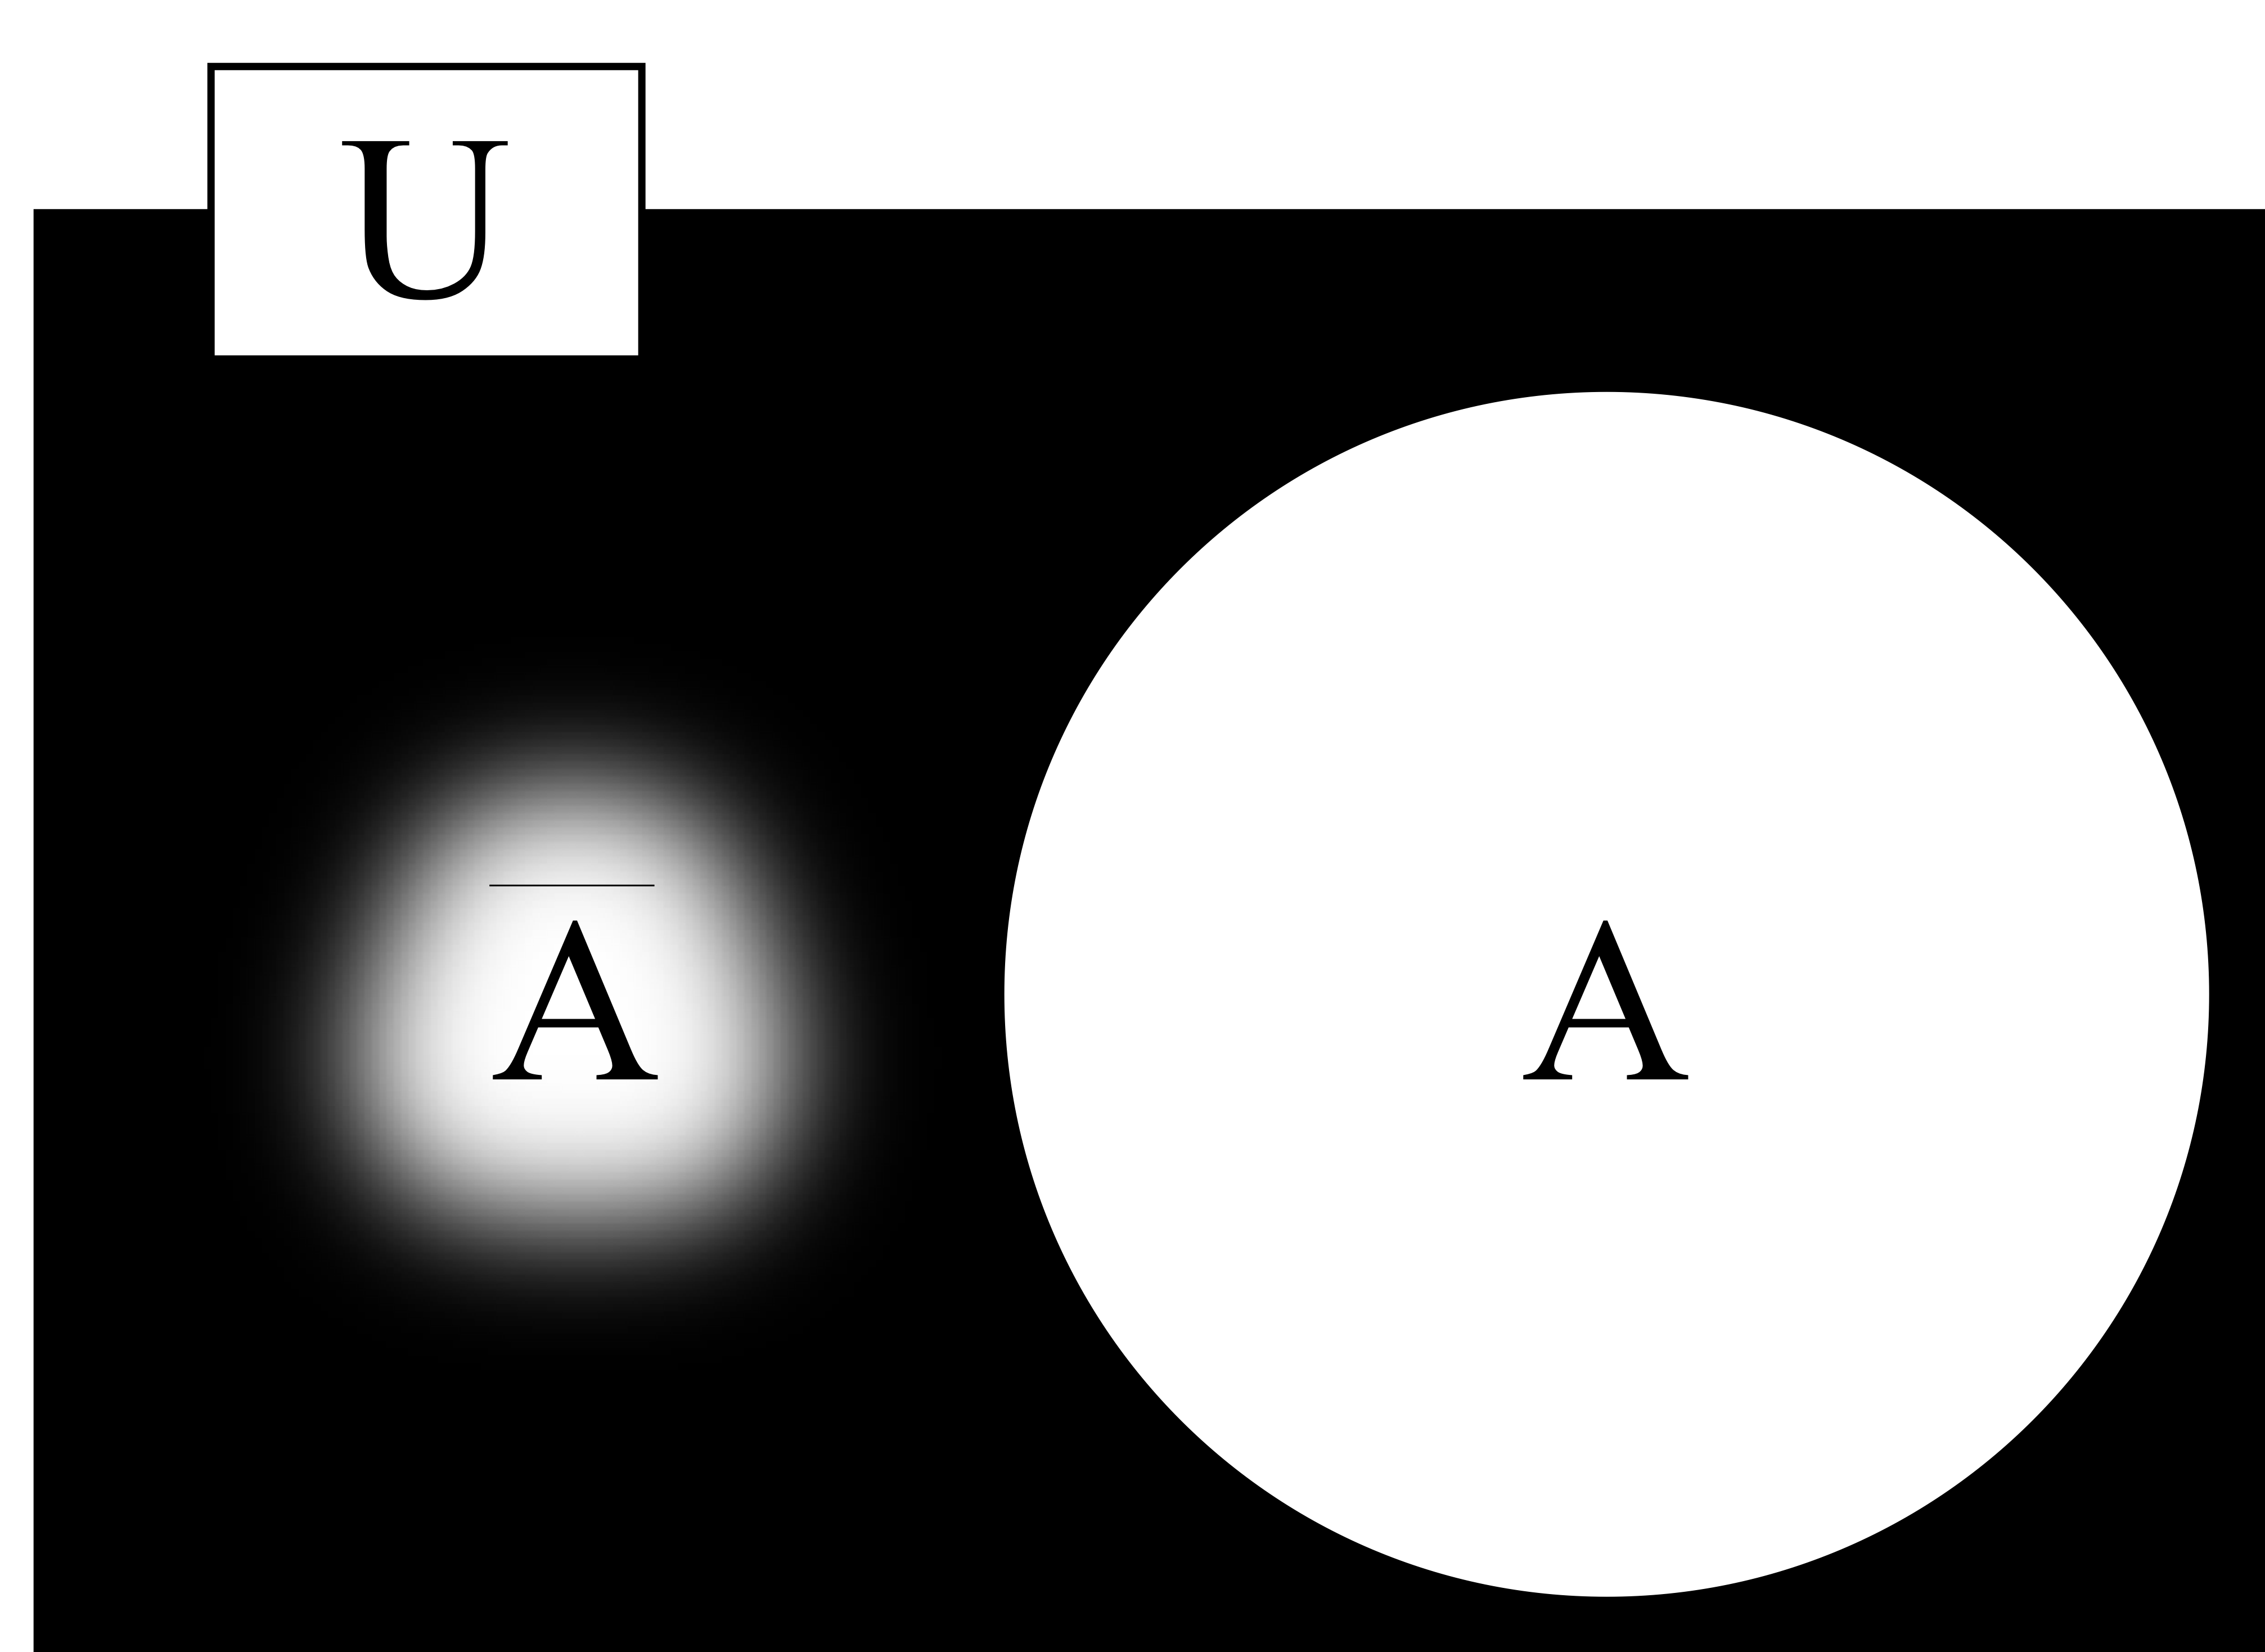
\includegraphics[width=8cm]{v1not.eps} \\%%% ファイル名
				\end {center}
			\end{minipage}
		\end{tabular}
		\caption{補集合のベン図}%%% 表題
		\label{fig:v1not}%%% ラベル
	\end{center}
\end{figure}
%
%
%
\begin{figure}[ht]
	\begin{center}
		\begin {tabular}{c}
			\begin{minipage}{8cm}
				\begin{center}
					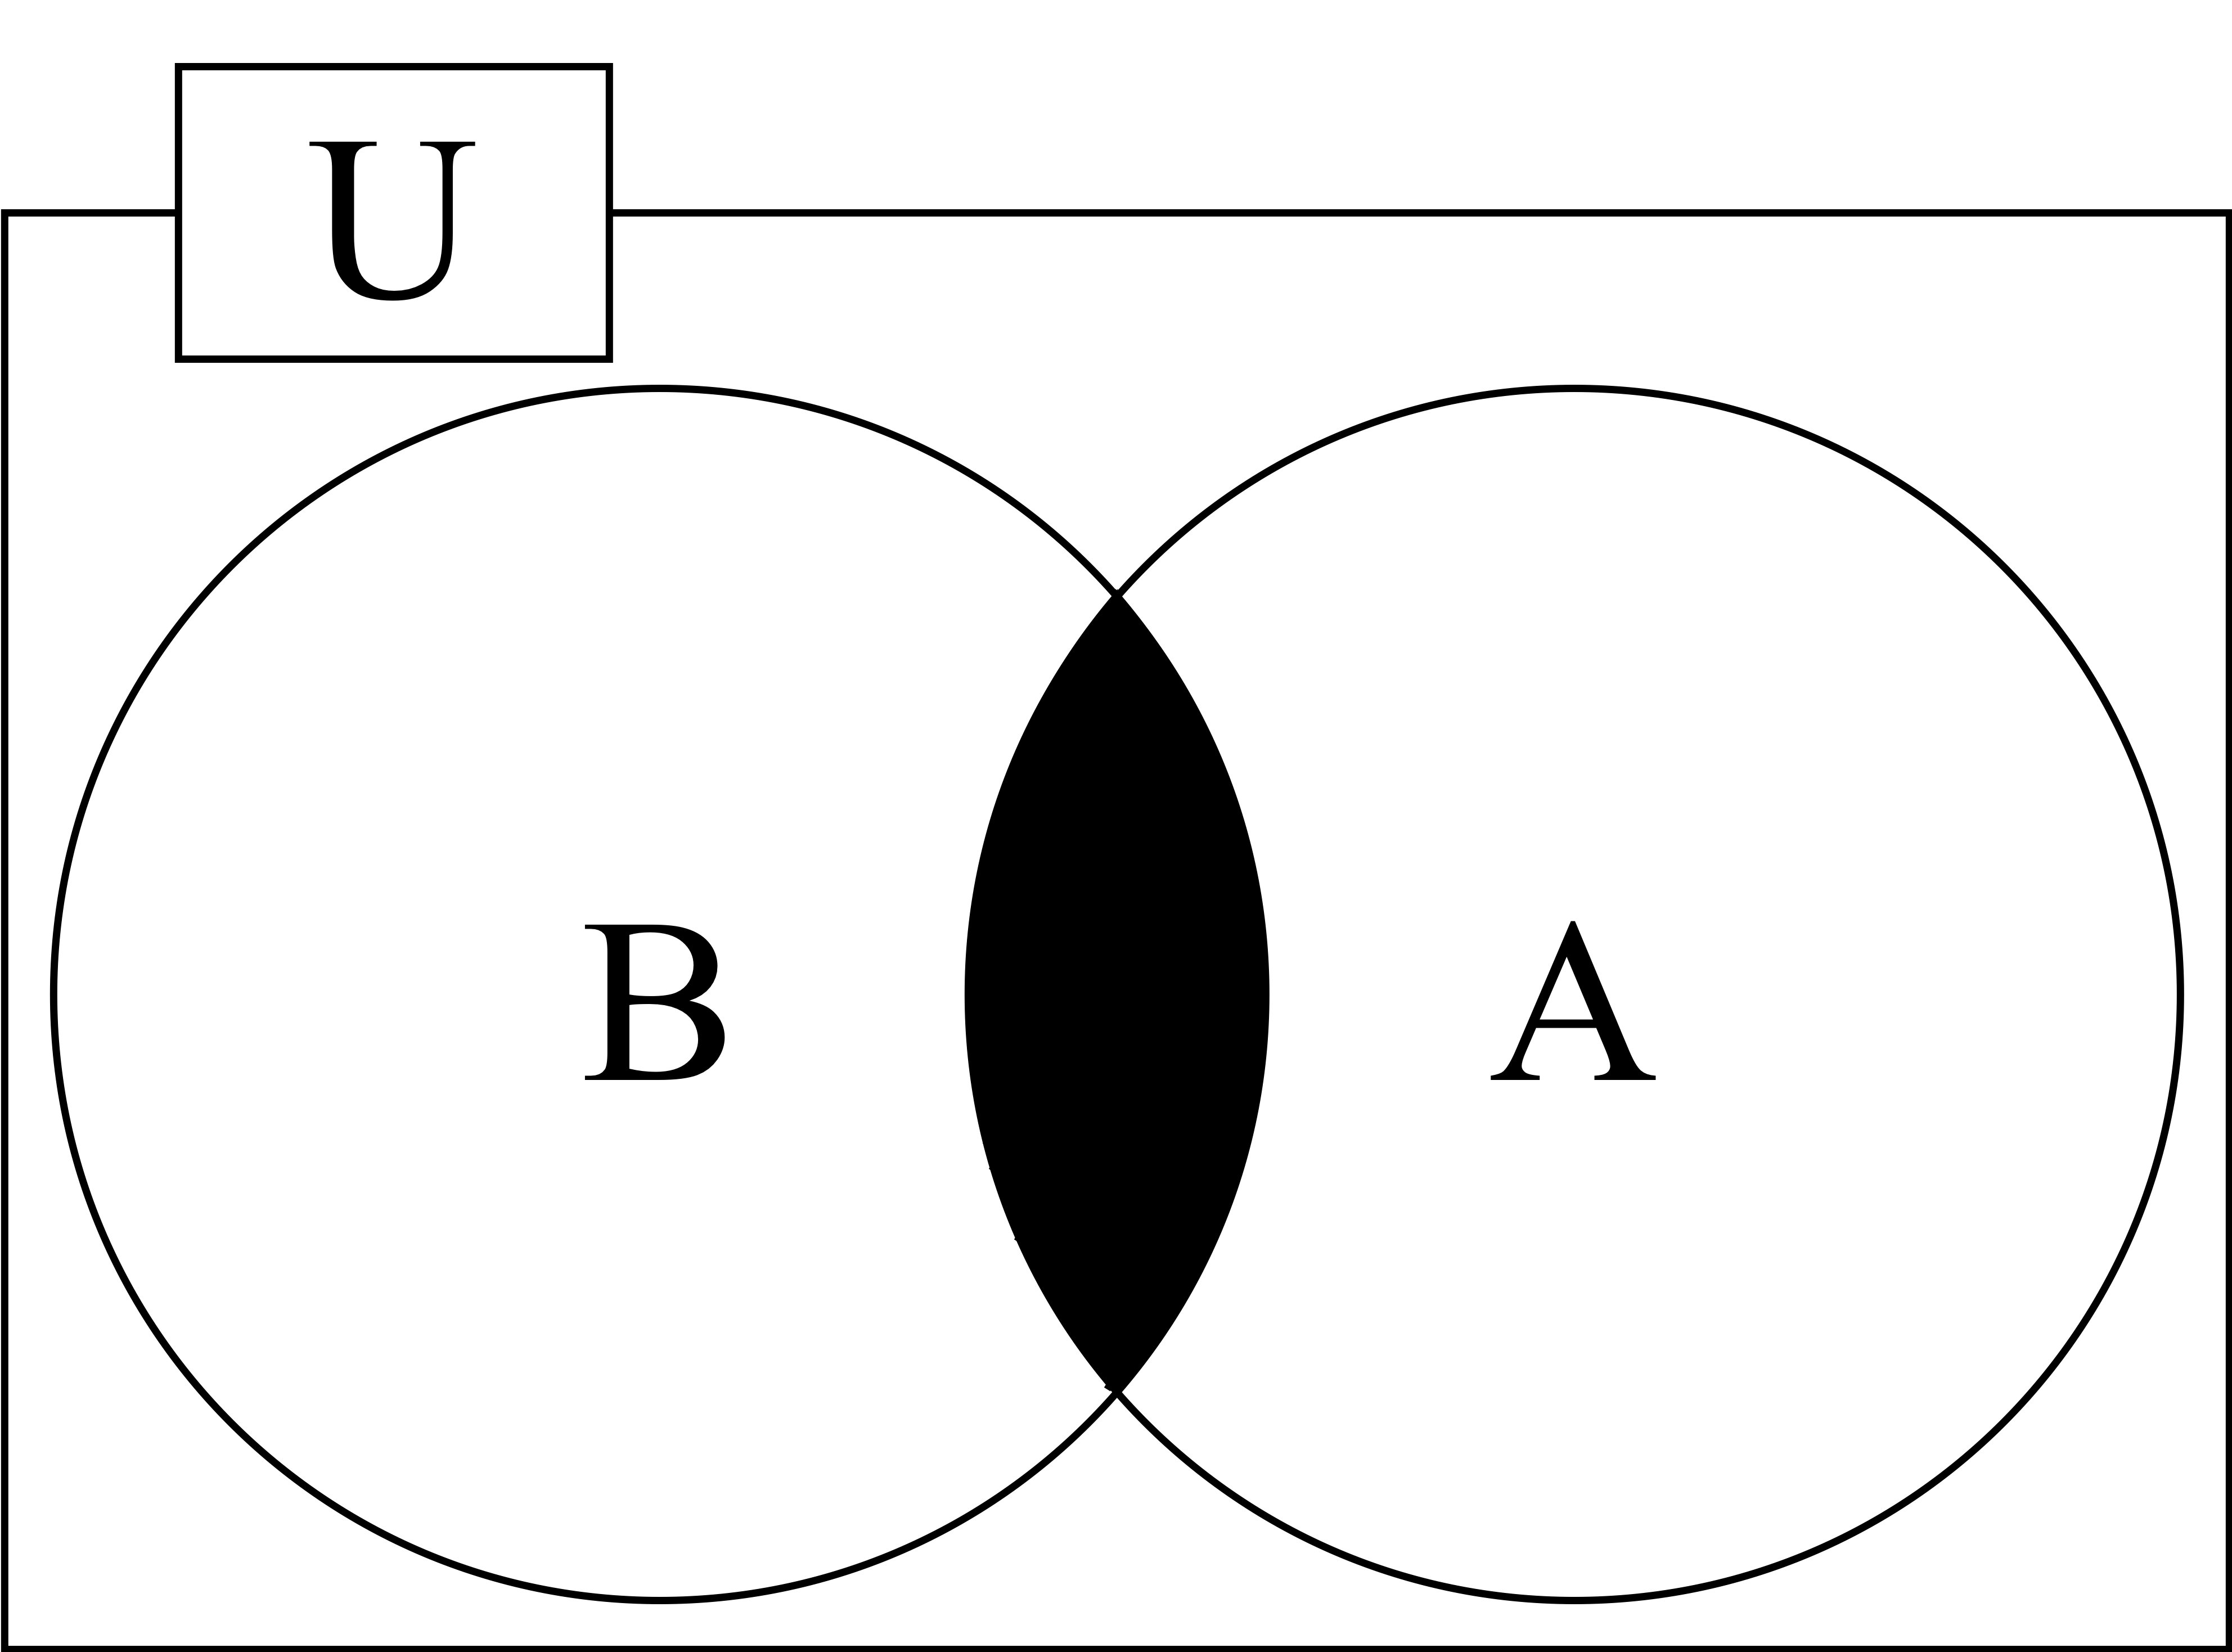
\includegraphics[width=8cm]{v2and.eps} \\%%% ファイル名
				\end {center}
			\end{minipage}
		\end{tabular}
		\caption{積集合のベン図}%%% 表題
		\label{fig:v2and}%%% ラベル
	\end{center}
\end{figure}
%
%
%
\begin{figure}[ht]
	\begin{center}
		\begin {tabular}{c}
			\begin{minipage}{8cm}
				\begin{center}
					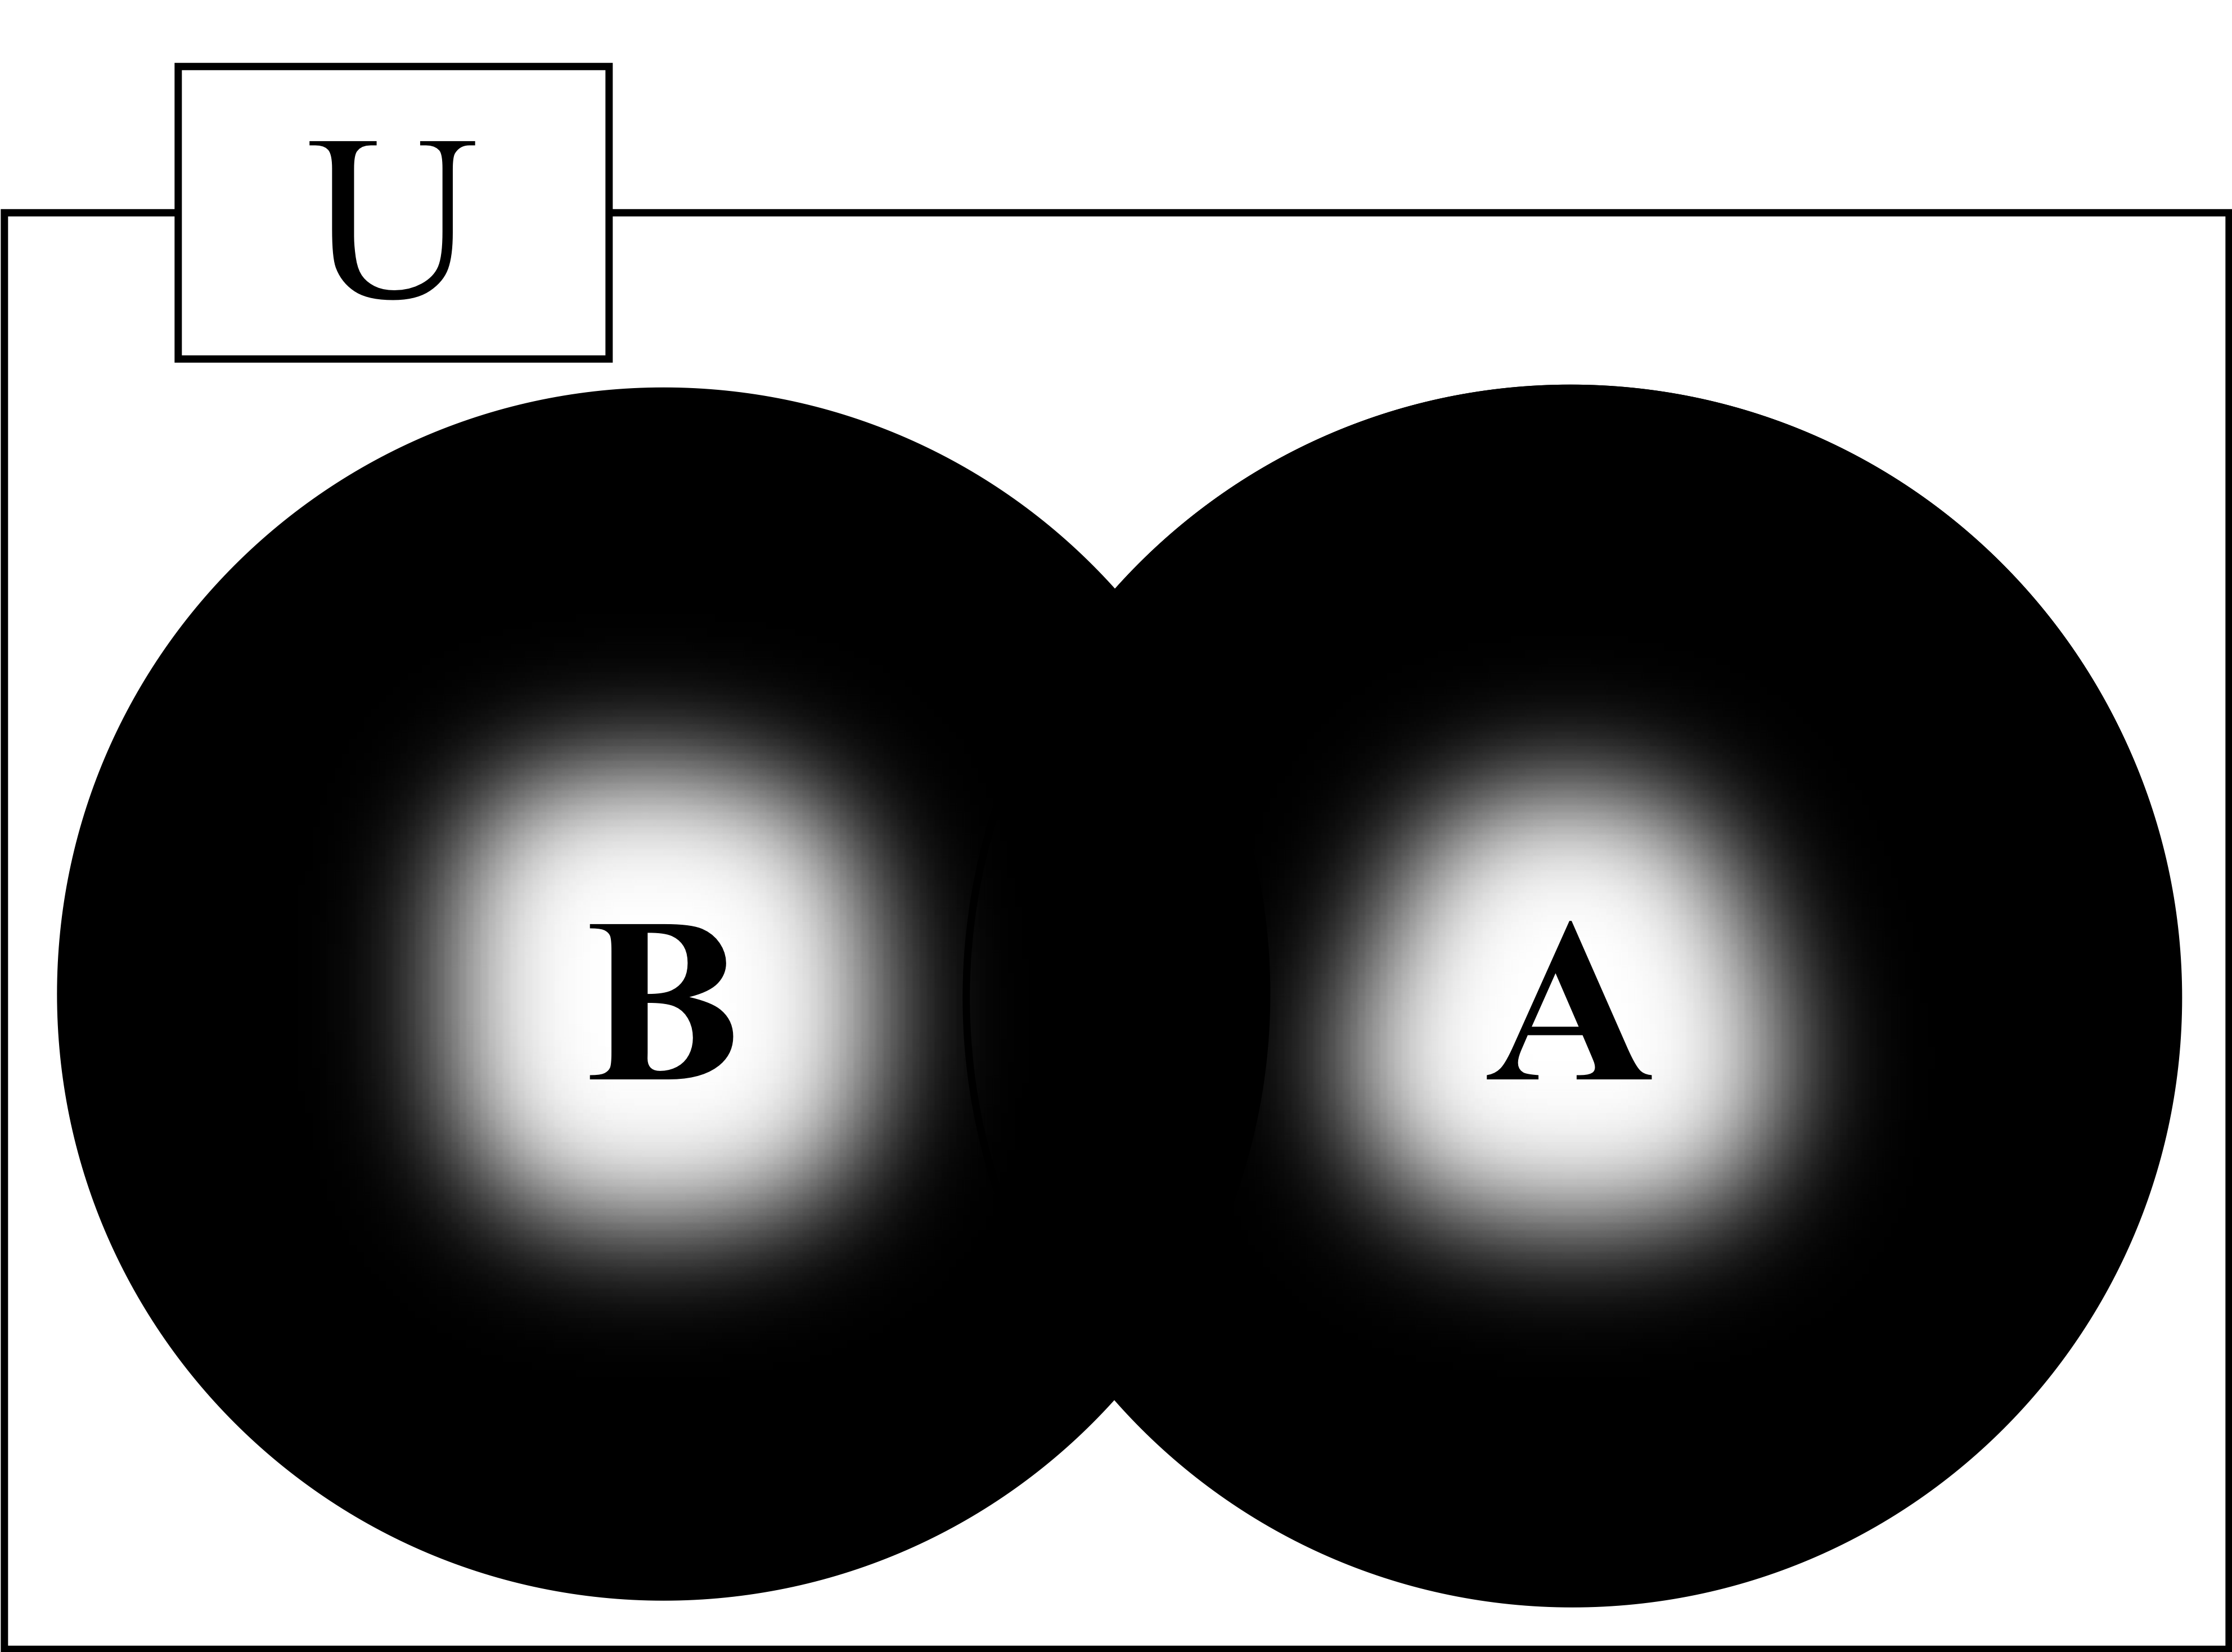
\includegraphics[width=8cm]{v3or.eps} \\%%% ファイル名
				\end {center}
			\end{minipage}
		\end{tabular}
		\caption{和集合のベン図}%%% 表題
		\label{fig:v3or}%%% ラベル
	\end{center}
\end{figure}
%
%
%
\begin{figure}[ht]
	\begin{center}
		\begin {tabular}{c}
			\begin{minipage}{8cm}
				\begin{center}
					\includegraphics[width=8cm]{v4nand.eps} \\%%% ファイル名
				\end {center}
			\end{minipage}
		\end{tabular}
		\caption{積集合の補集合のベン図}%%% 表題
		\label{fig:v4nand}%%% ラベル
	\end{center}
\end{figure}
%
%
%
\begin{figure}[ht]
	\begin{center}
		\begin {tabular}{c}
			\begin{minipage}{8cm}
				\begin{center}
					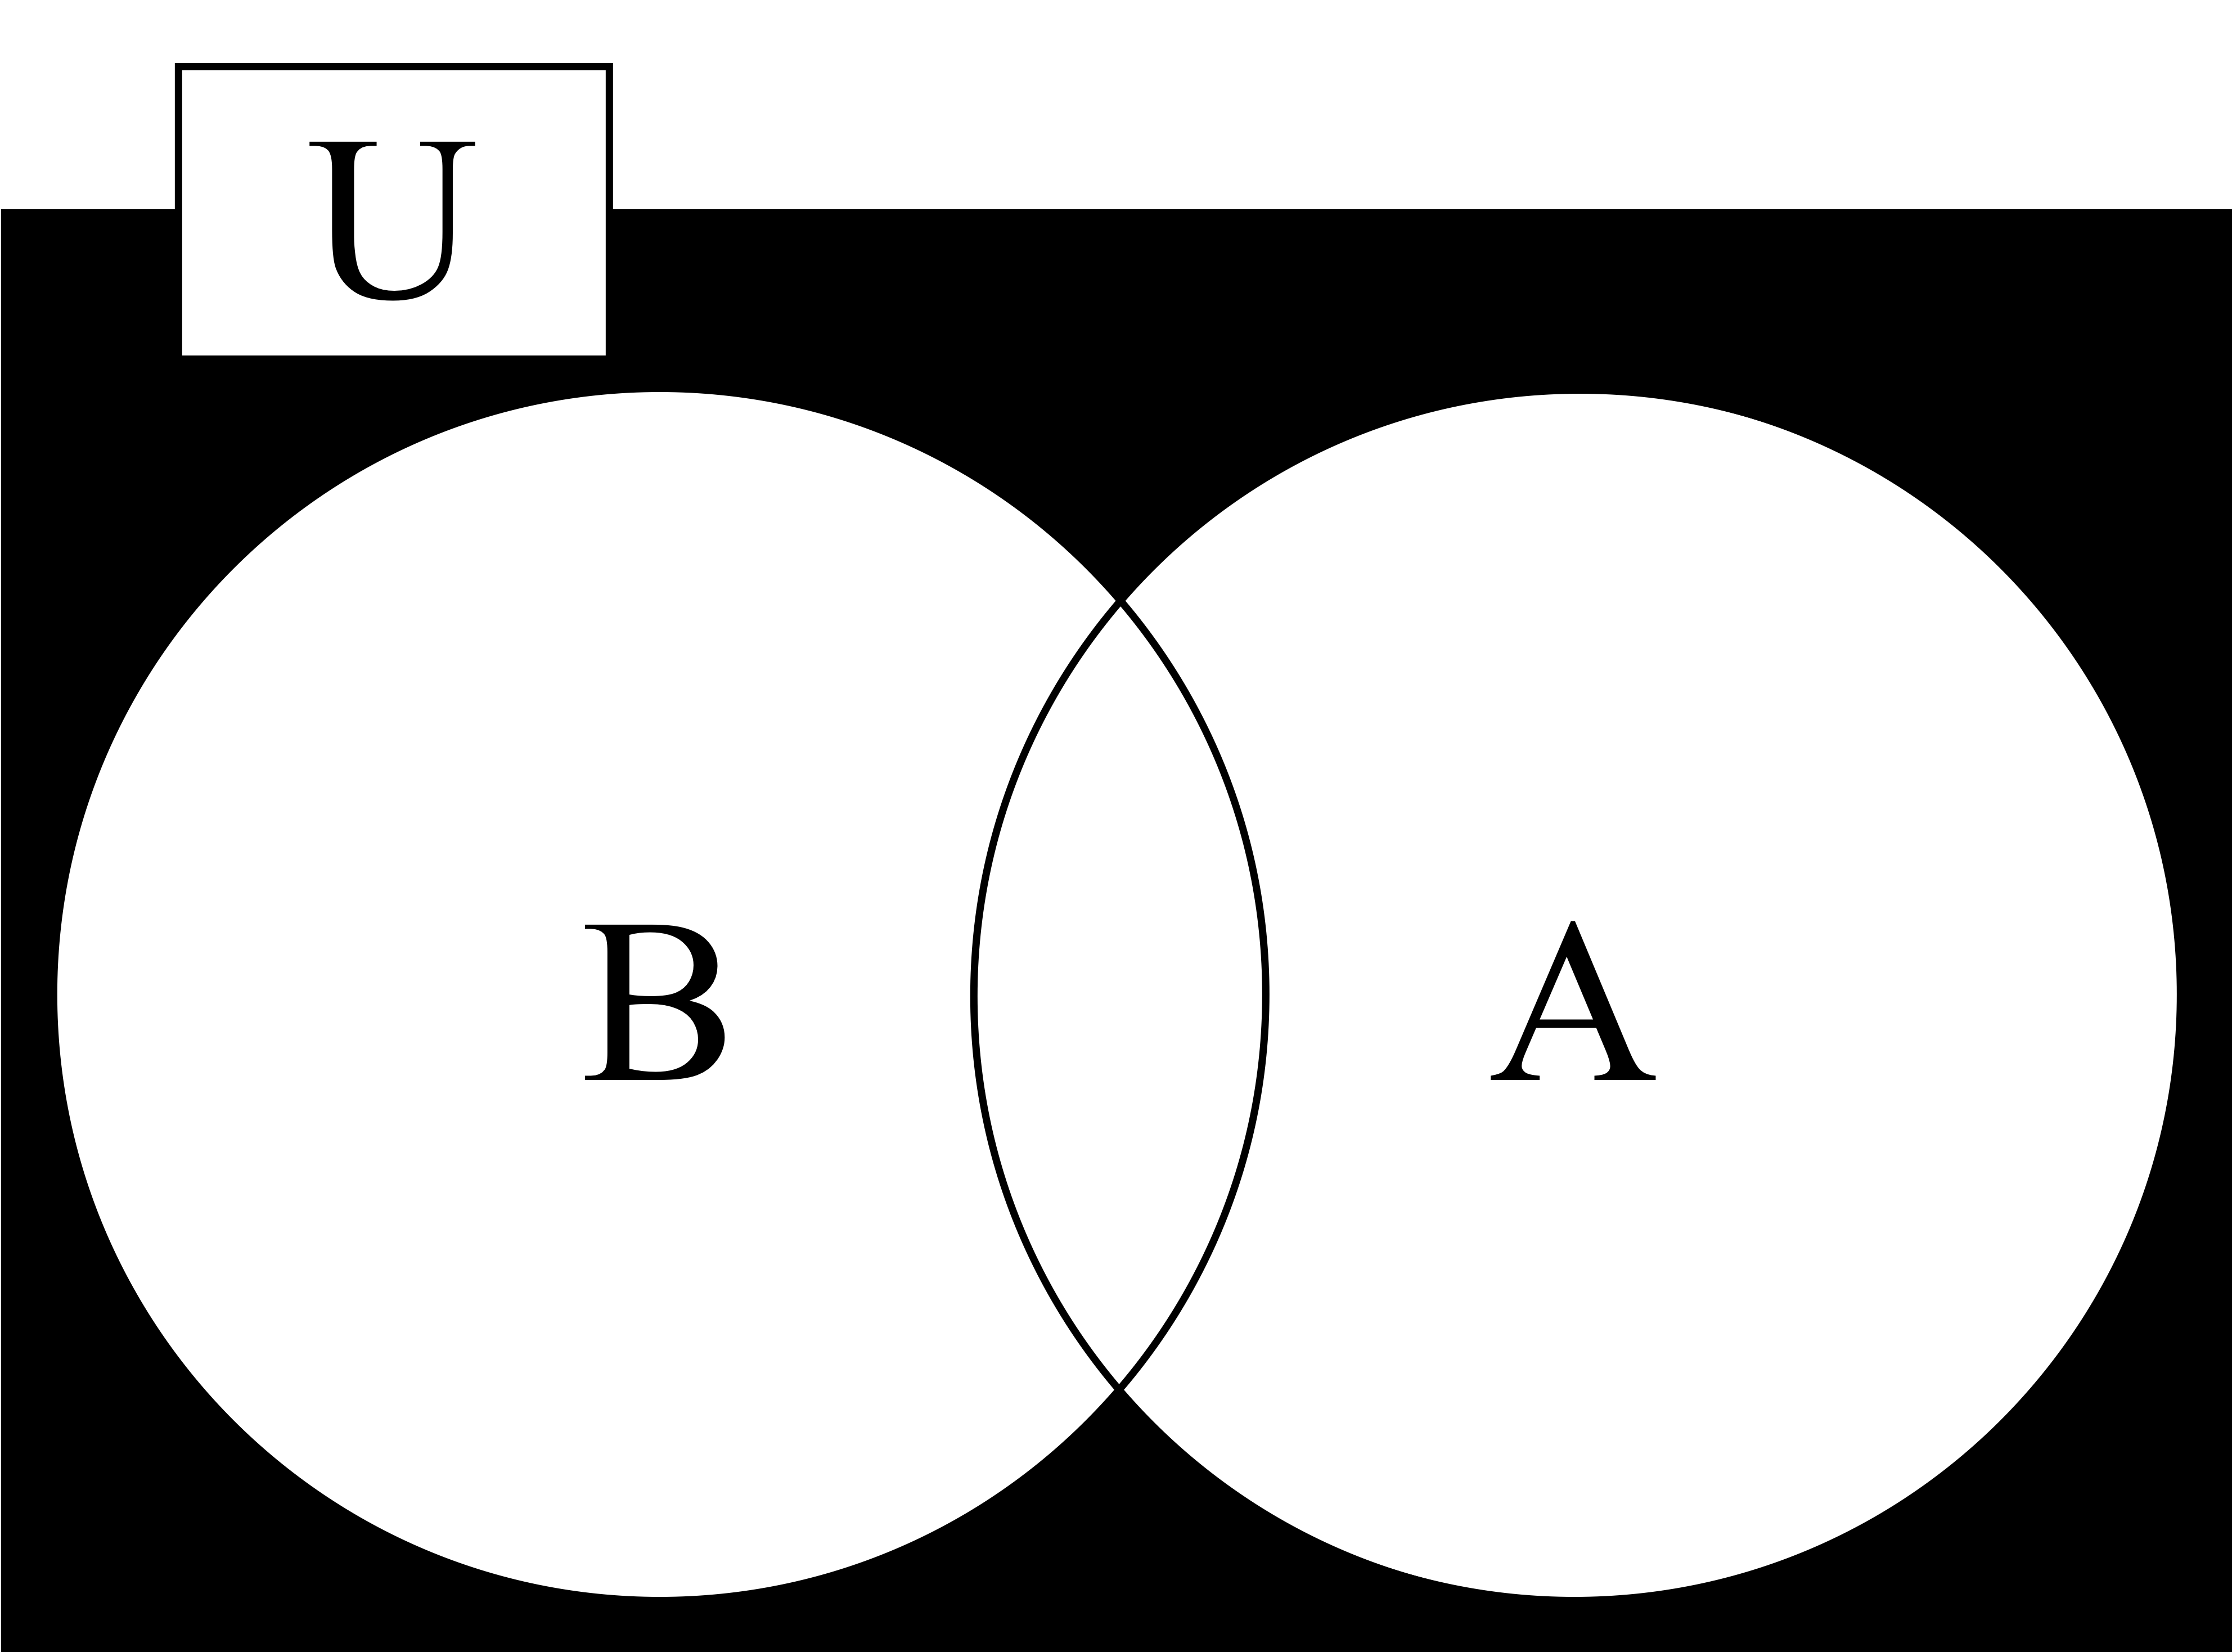
\includegraphics[width=8cm]{v5nor.eps} \\%%% ファイル名
				\end {center}
			\end{minipage}
		\end{tabular}
		\caption{和集合の補集合ベン図}%%% 表題
		\label{fig:v5nor}%%% ラベル
	\end{center}
\end{figure}
%
%
%
\begin{figure}[ht]
	\begin{center}
		\begin {tabular}{c}
			\begin{minipage}{8cm}
				\begin{center}
					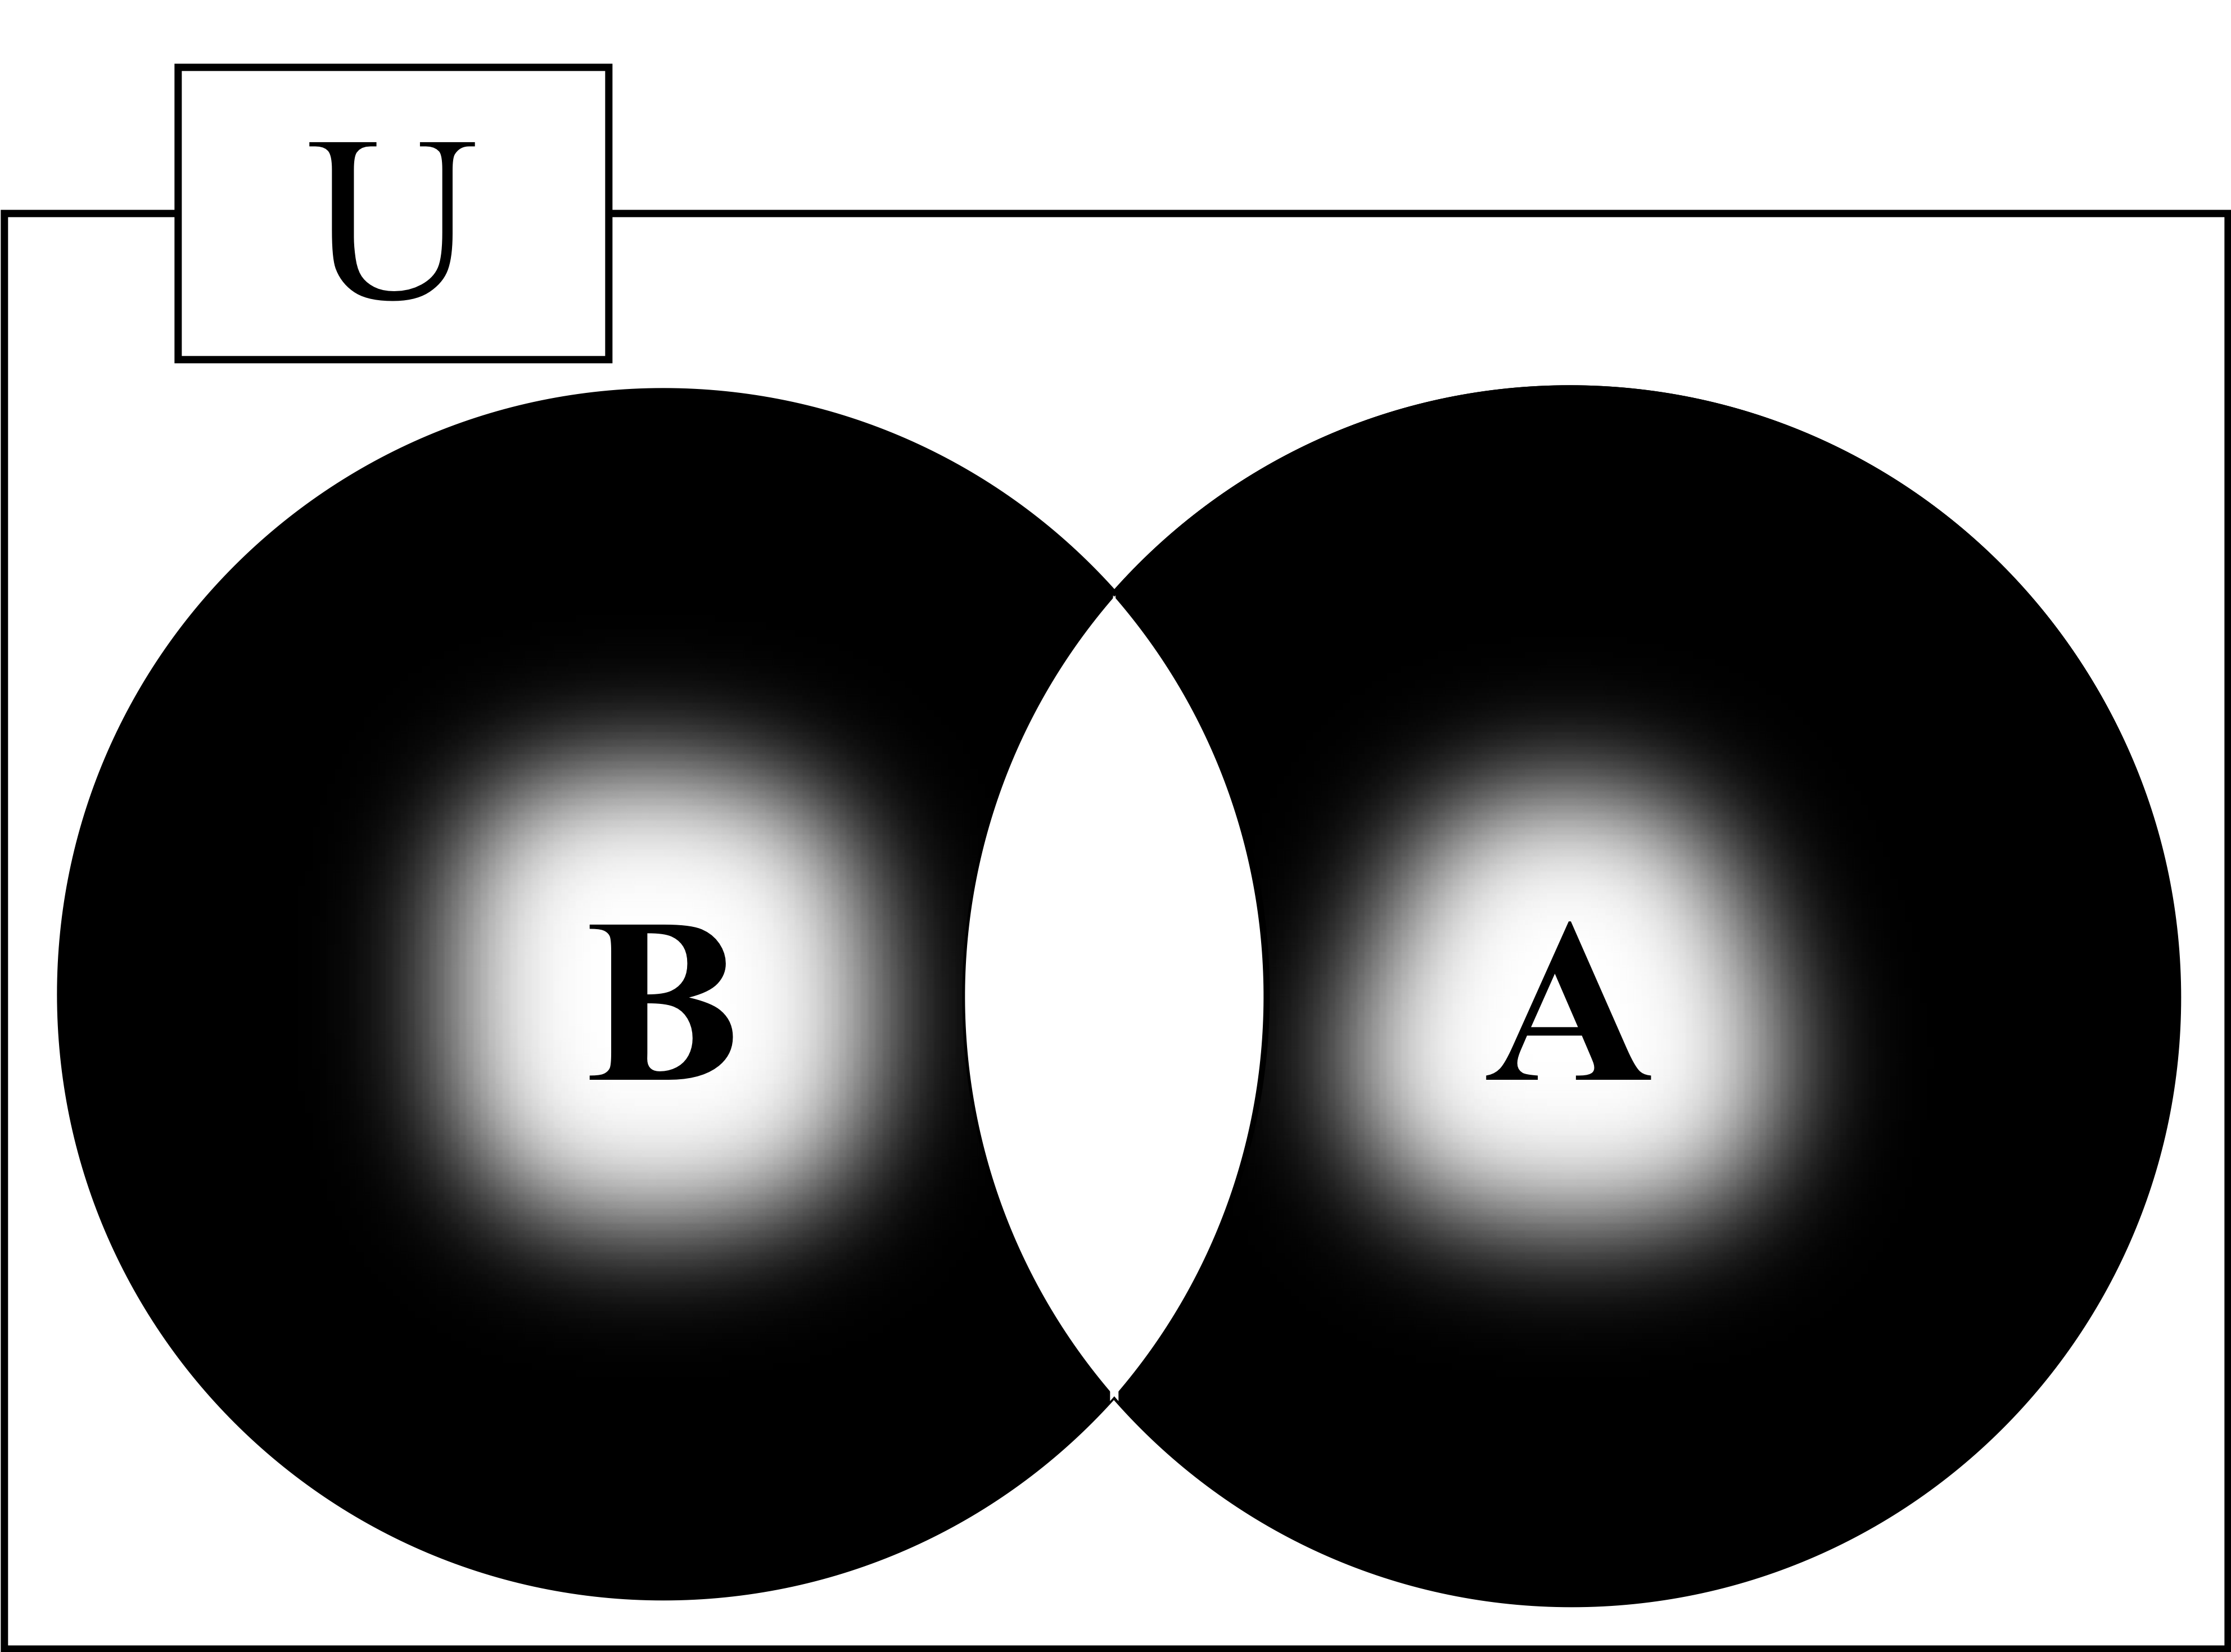
\includegraphics[width=8cm]{v6exor.eps} \\%%% ファイル名
				\end {center}
			\end{minipage}
		\end{tabular}
		\caption{排他的論理和のベン図}%%% 表題
		\label{fig:v6exor}%%% ラベル
	\end{center}
\end{figure}
%
%
%
\begin{figure}[ht]
	\begin{center}
		\begin {tabular}{c}
			\begin{minipage}{8cm}
				\begin{center}
					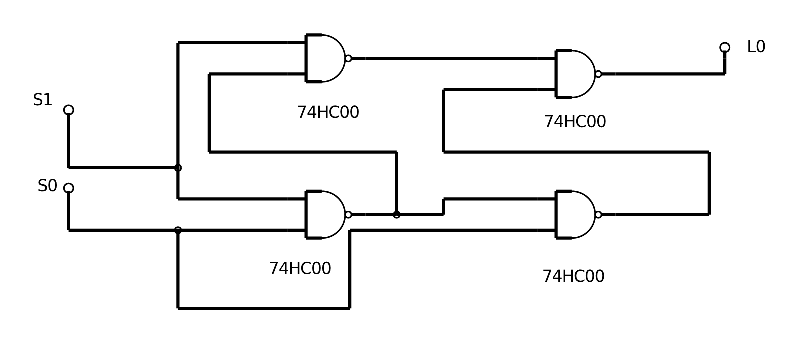
\includegraphics[width=8cm]{exor} \\%%% ファイル名
				\end {center}
			\end{minipage}
		\end{tabular}
		\caption{$2$入力ExOR回路の回路図}%%% 表題
		\label{fig:ExOR}%%% ラベル
	\end{center}
\end{figure}
%
%
%
\begin{figure}[ht]
	\begin{center}
		\begin {tabular}{c}
			\begin{minipage}{8cm}
				\begin{center}
					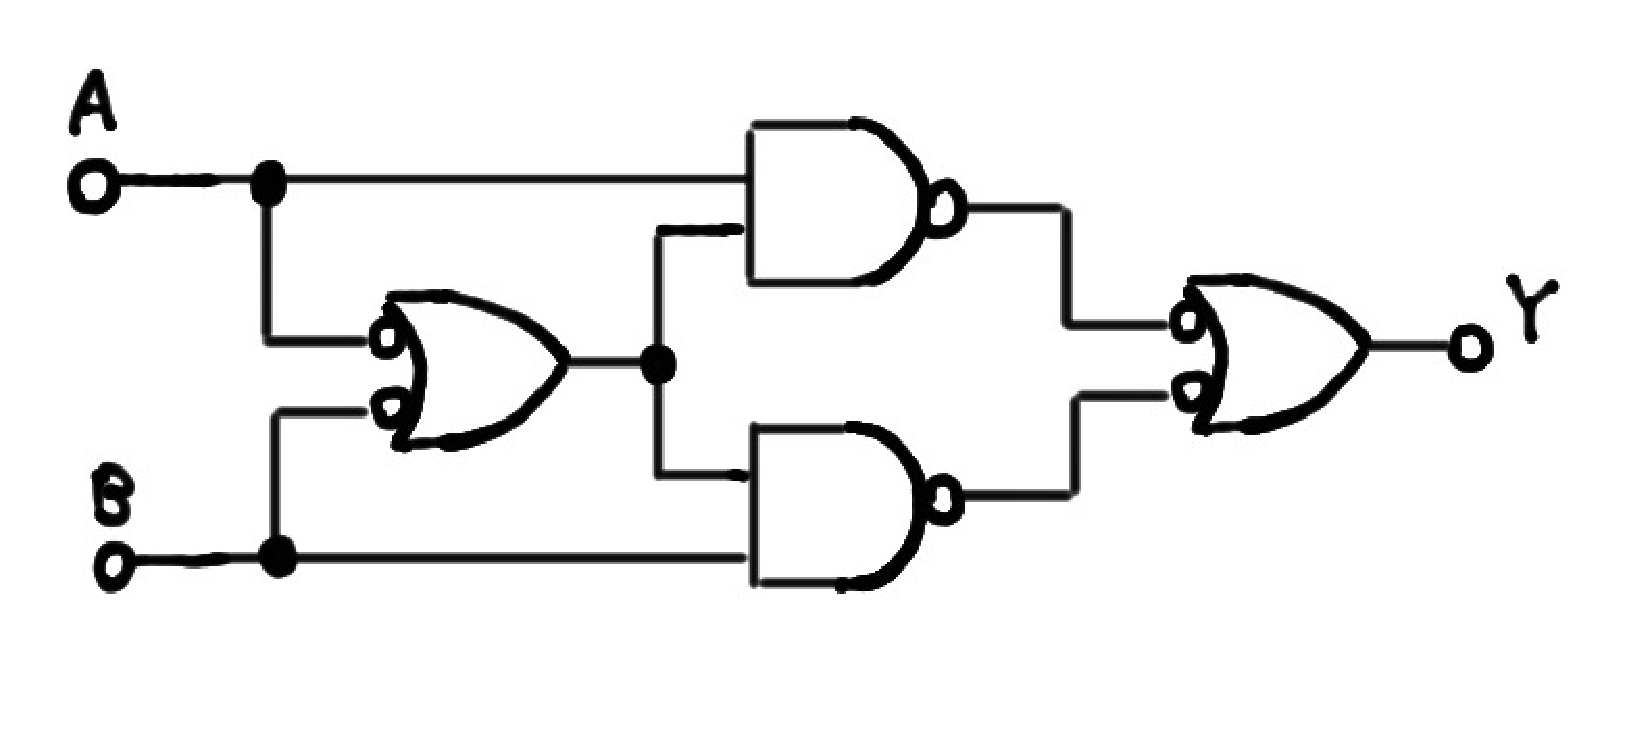
\includegraphics[width=8cm]{exor22} \\%%% ファイル名
				\end {center}
			\end{minipage}
		\end{tabular}
		\caption{課題1におけるExOR回路の回路図}%%% 表題
		\label{fig:ExOR_kadai1}%%% ラベル
	\end{center}
\end{figure}
%
%
%
\begin{figure}[ht]
	\begin{center}
		\begin {tabular}{c}
			\begin{minipage}{8cm}
				\begin{center}
					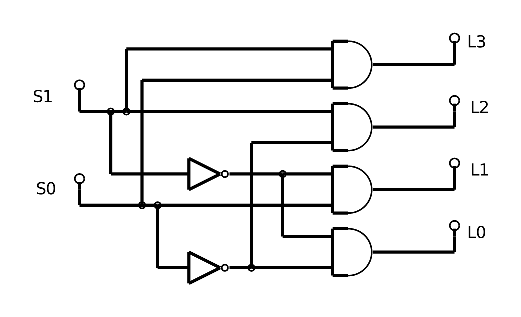
\includegraphics[width=8cm]{24decoder} \\%%% ファイル名
				\end {center}
			\end{minipage}
		\end{tabular}
		\caption{$2$入力$4$出力デコーダの回路図}%%% 表題
		\label{fig:24decoder}%%% ラベル
	\end{center}
\end{figure}
%
%
%
\begin{figure}[ht]
	\begin{center}
		\begin {tabular}{c}
			\begin{minipage}{8cm}
				\begin{center}
					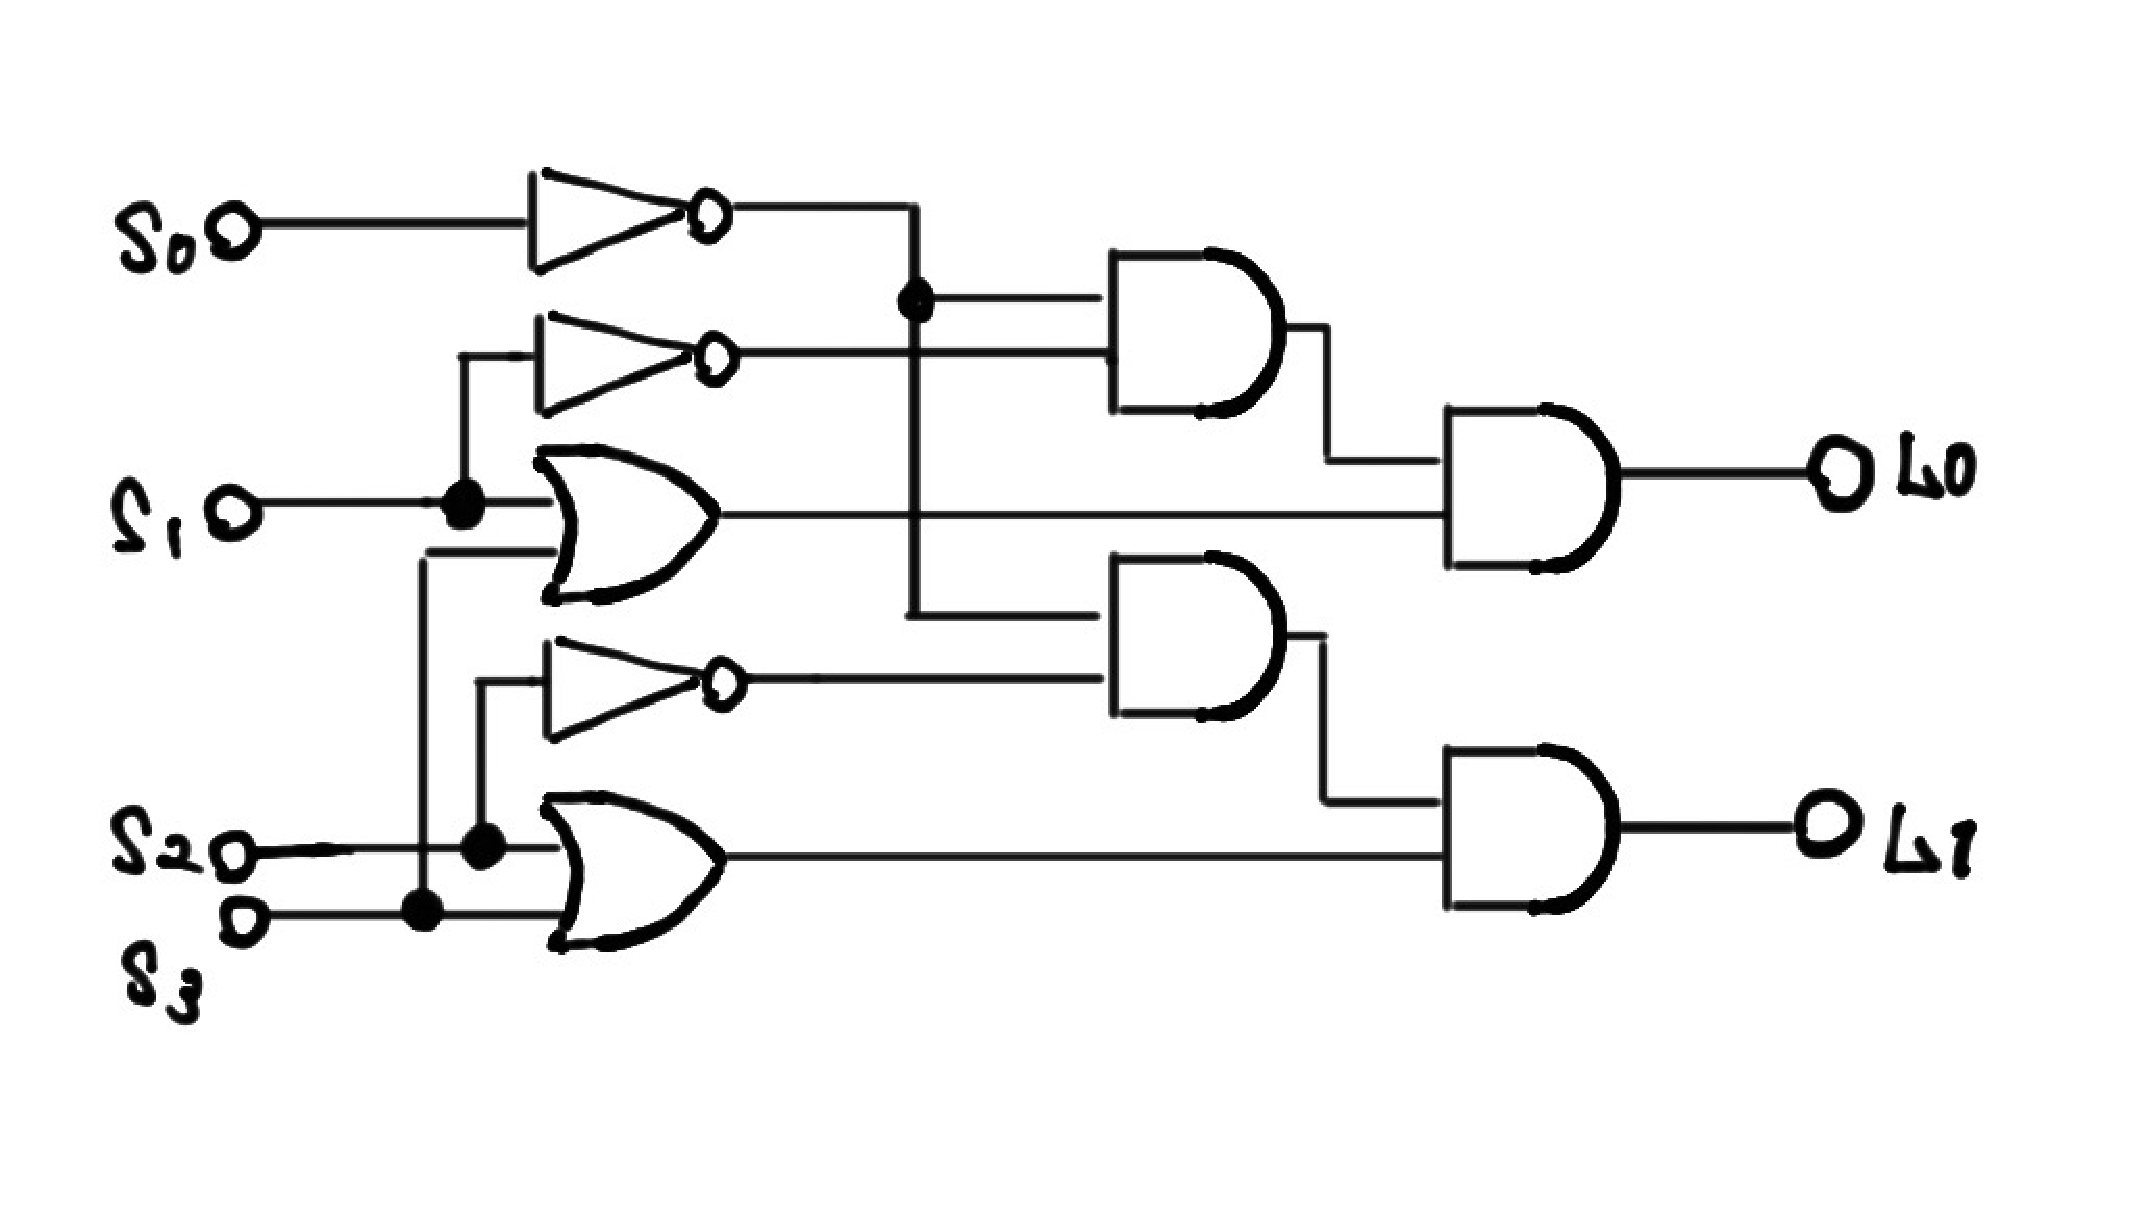
\includegraphics[width=8cm]{halfadder3} \\%%% ファイル名
				\end {center}
			\end{minipage}
		\end{tabular}
		\caption{$4$入力$2$出力エンコーダの回路図(複数選択可能)}%%% 表題
		\label{fig:42encodern}%%% ラベル
	\end{center}
\end{figure}

\begin{figure}[ht]
	\begin{center}
		\begin {tabular}{c}
			\begin{minipage}{8cm}
				\begin{center}
					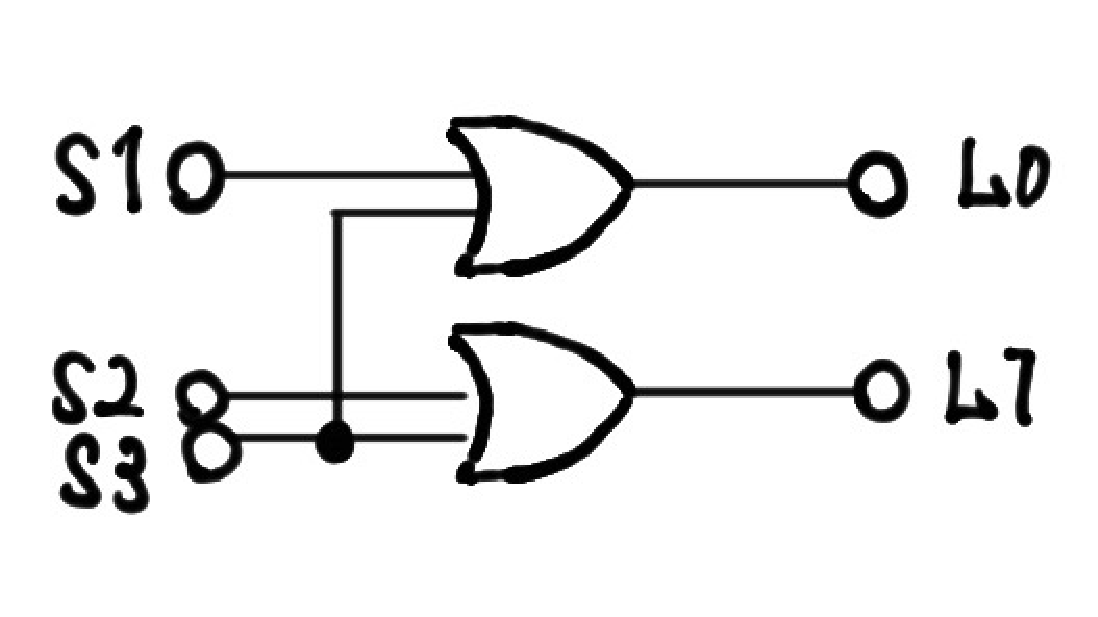
\includegraphics[width=8cm]{halfadder2} \\%%% ファイル名
				\end {center}
			\end{minipage}
		\end{tabular}
		\caption{$4$入力$2$出力エンコーダの回路図(選択が1つしかできない場合)}%%% 表題
		\label{fig:42encoder1}%%% ラベル
	\end{center}
\end{figure}
%
%
%
\begin{figure}[ht]
	\begin{center}
		\begin {tabular}{c}
			\begin{minipage}{8cm}
				\begin{center}
					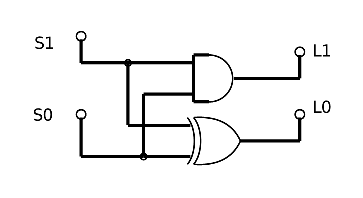
\includegraphics[width=8cm]{halfadder} \\%%% ファイル名
				\end {center}
			\end{minipage}
		\end{tabular}
		\caption{半加算器回路の回路図}%%% 表題
		\label{fig:halfAdder}%%% ラベル
	\end{center}
\end{figure}
%
%
%
\begin{figure}[ht]
	\begin{center}
		\begin {tabular}{c}
			\begin{minipage}{8cm}
				\begin{center}
					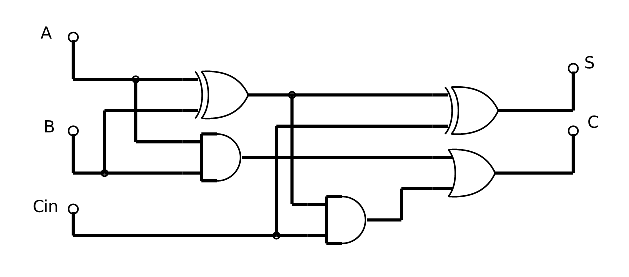
\includegraphics[width=8cm]{fulladder} \\%%% ファイル名
				\end {center}
			\end{minipage}
		\end{tabular}
		\caption{全加算器回路の回路図}%%% 表題
		\label{fig:fullAdder}%%% ラベル
	\end{center}
\end{figure}
%
%
%
\begin{figure}[ht]
	\begin{center}
		\begin {tabular}{c}
			\begin{minipage}{8cm}
				\begin{center}
					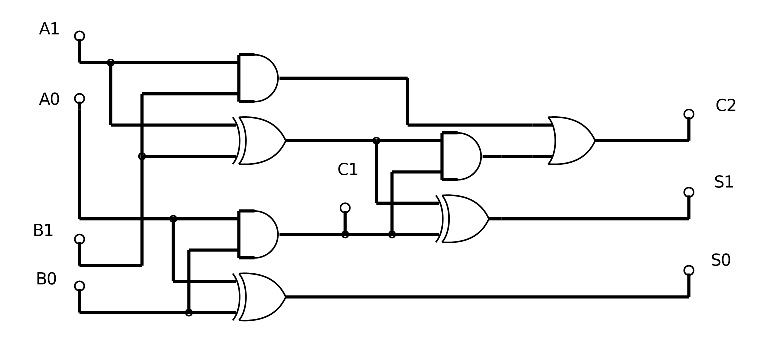
\includegraphics[width=8cm]{22adder} \\%%% ファイル名
				\end {center}
			\end{minipage}
		\end{tabular}
		\caption{2桁の2進数の加算器回路の回路図}%%% 表題
		\label{fig:22Adder}%%% ラベル
	\end{center}
\end{figure}
%
%
%
\begin{figure}[ht]
	\begin{center}
		\begin {tabular}{c}
			\begin{minipage}{8cm}
				\begin{center}
					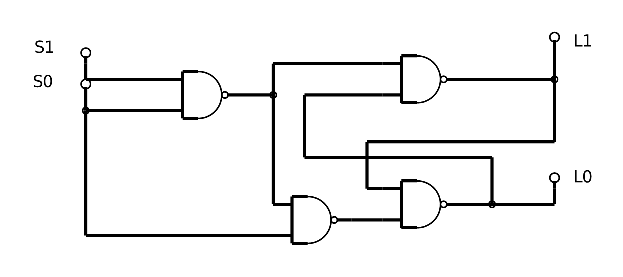
\includegraphics[width=8cm]{Dlatch} \\%%% ファイル名
				\end {center}
			\end{minipage}
		\end{tabular}
		\caption{Dラッチ回路の回路図}%%% 表題
		\label{fig:DLatch}%%% ラベル
	\end{center}
\end{figure}
%
%
%
\begin{figure}[ht]
	\begin{center}
		\begin {tabular}{c}
			\begin{minipage}{8cm}
				\begin{center}
					\includegraphics[width=8cm]{DlatchTC} \\%%% ファイル名
				\end {center}
			\end{minipage}
		\end{tabular}
		\caption{Dラッチ回路のタイムチャート}%%% 表題
		\label{fig:DLatchTC}%%% ラベル
	\end{center}
\end{figure}
%
%
%
\begin{figure}[ht]
	\begin{center}
		\begin {tabular}{c}
			\begin{minipage}{8cm}
				\begin{center}
					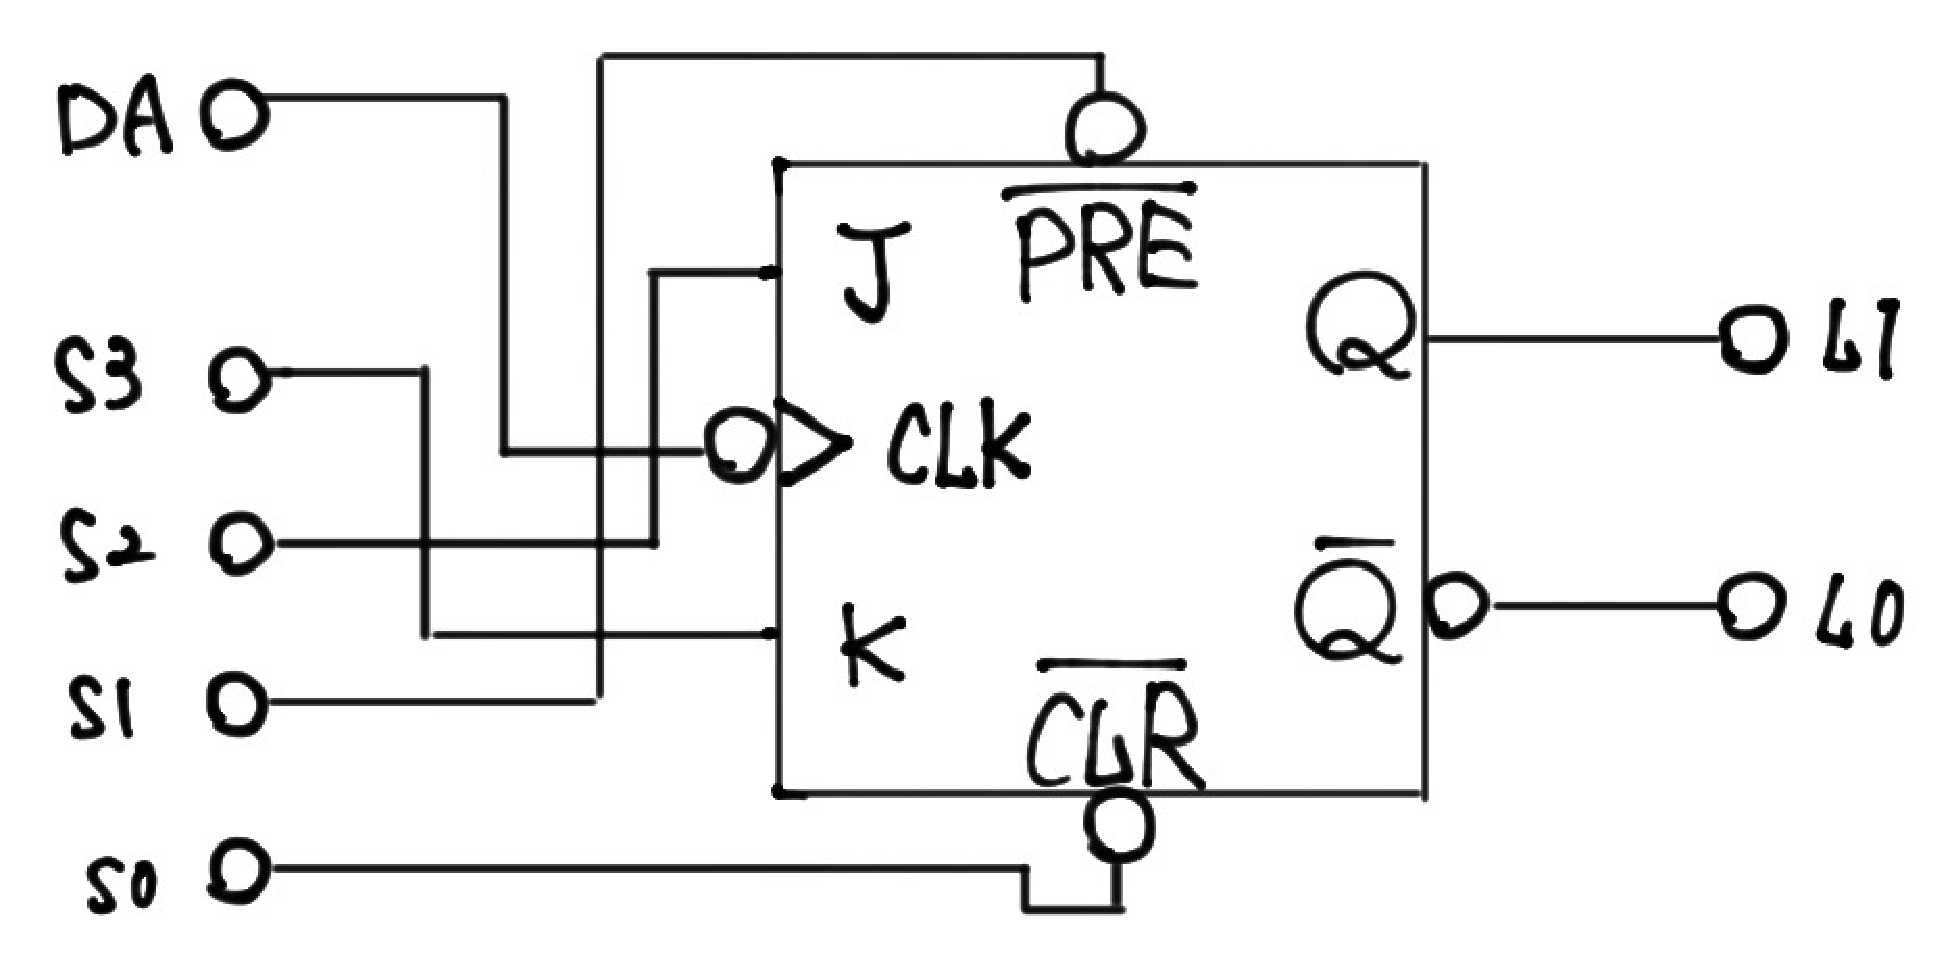
\includegraphics[width=8cm]{jkffcirc2} \\%%% ファイル名
				\end {center}
			\end{minipage}
		\end{tabular}
		\caption{J-Kフリップフロップ回路の回路図}%%% 表題
		\label{fig:JKFF}%%% ラベル
	\end{center}
\end{figure}
%
%
%
\begin{figure}[ht]
	\begin{center}
		\begin {tabular}{c}
			\begin{minipage}{8cm}
				\begin{center}
					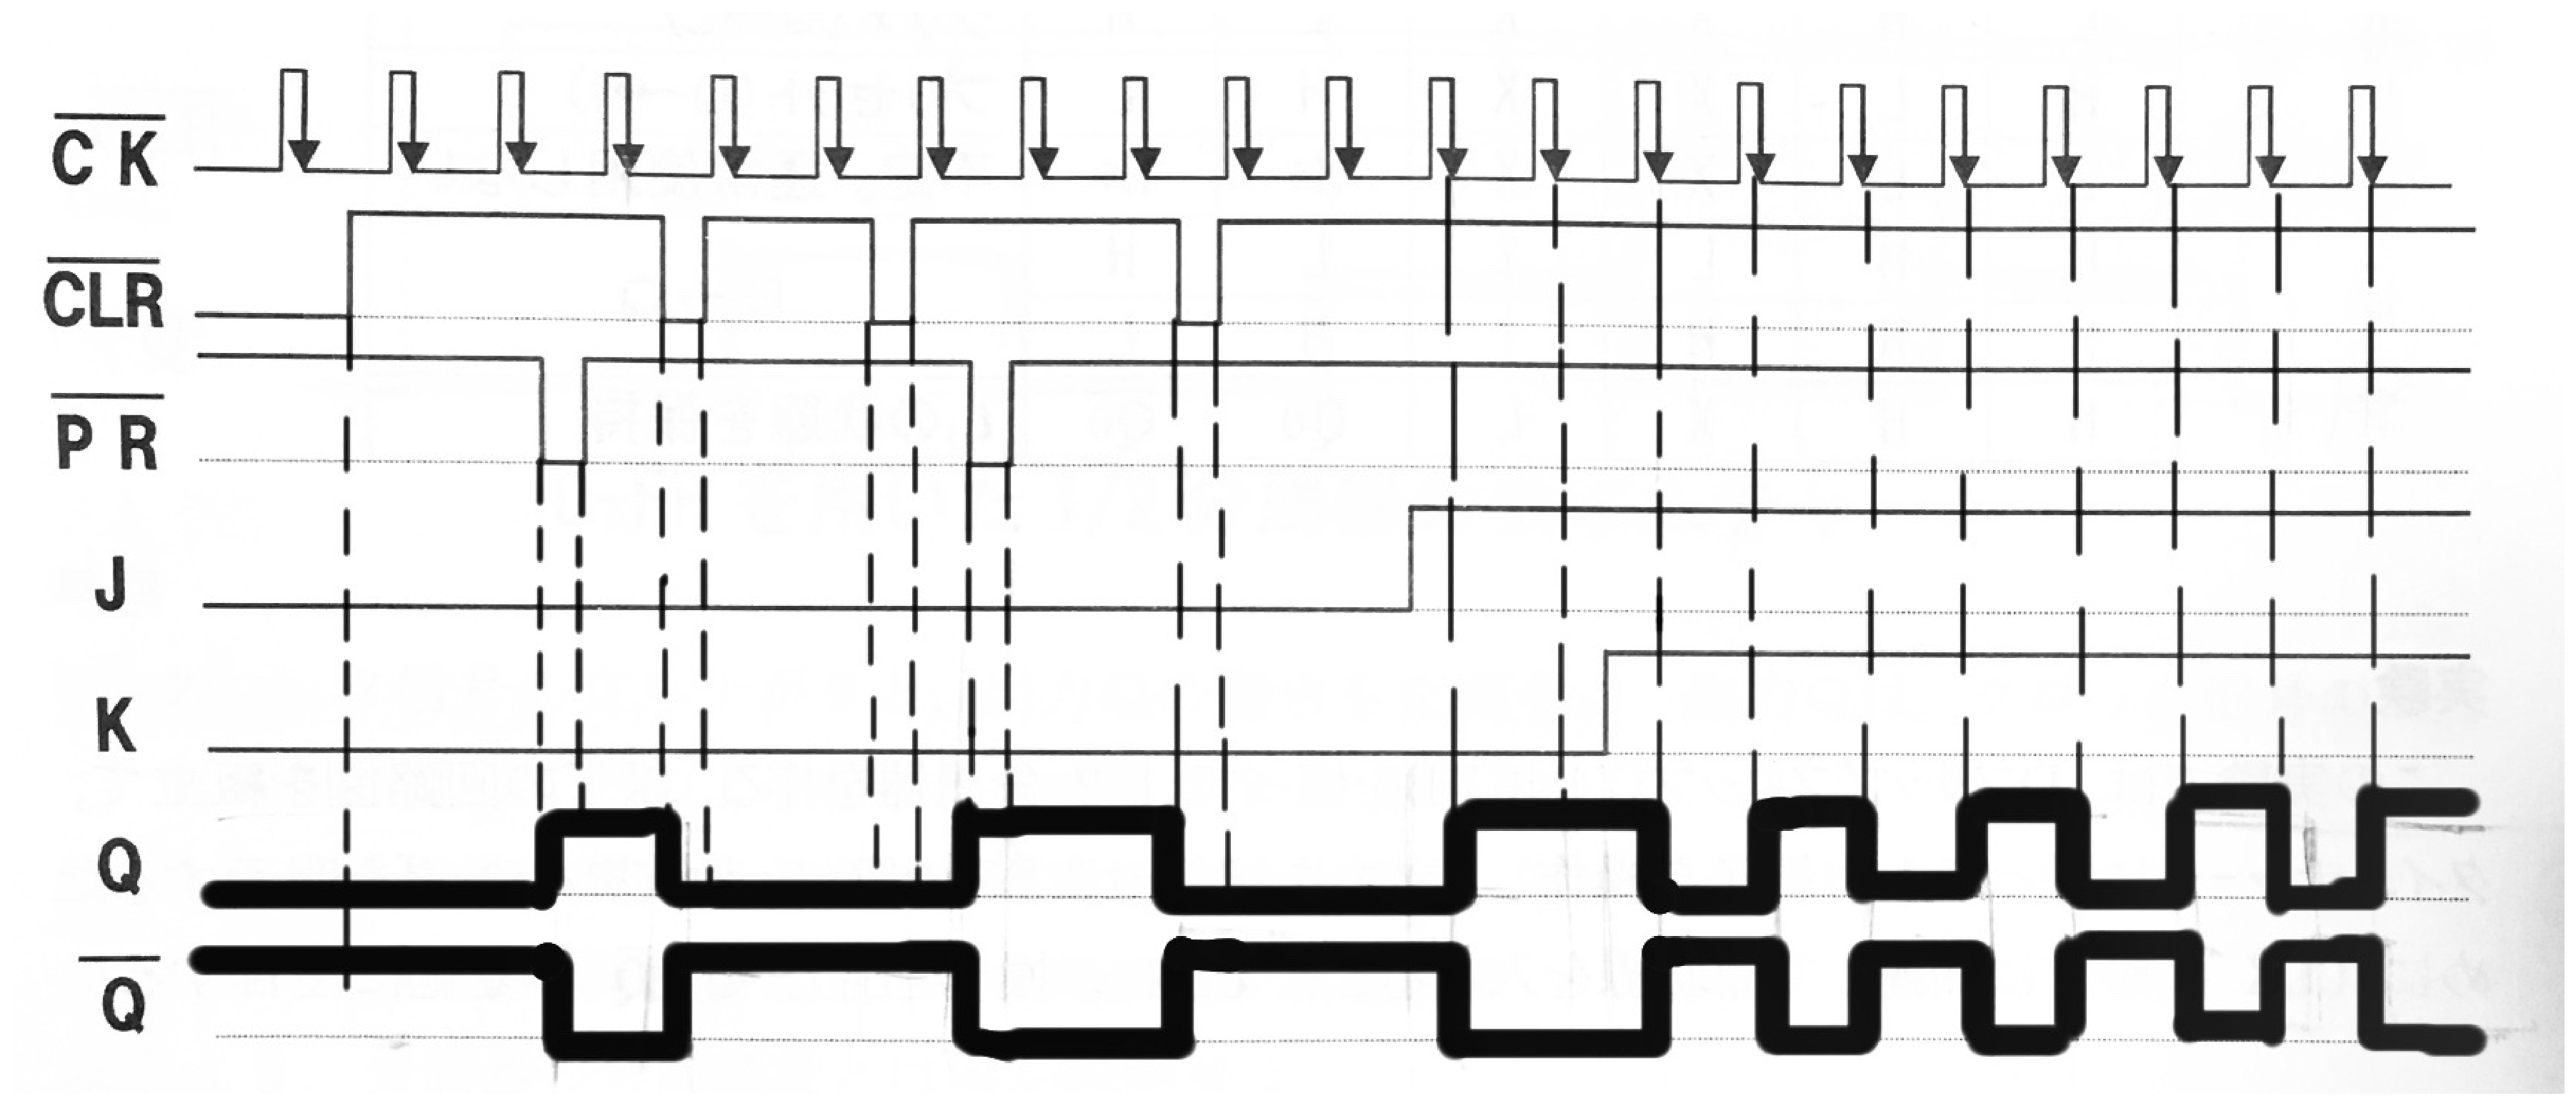
\includegraphics[width=8cm]{jkff2} \\%%% ファイル名
				\end {center}
			\end{minipage}
		\end{tabular}
		\caption{J-Kフリップフロップ回路のタイムチャート}%%% 表題
		\label{fig:JKFFTC}%%% ラベル
	\end{center}
\end{figure}
%
%
%
\begin{figure}[ht]
	\begin{center}
		\begin {tabular}{c}
			\begin{minipage}{8cm}
				\begin{center}
					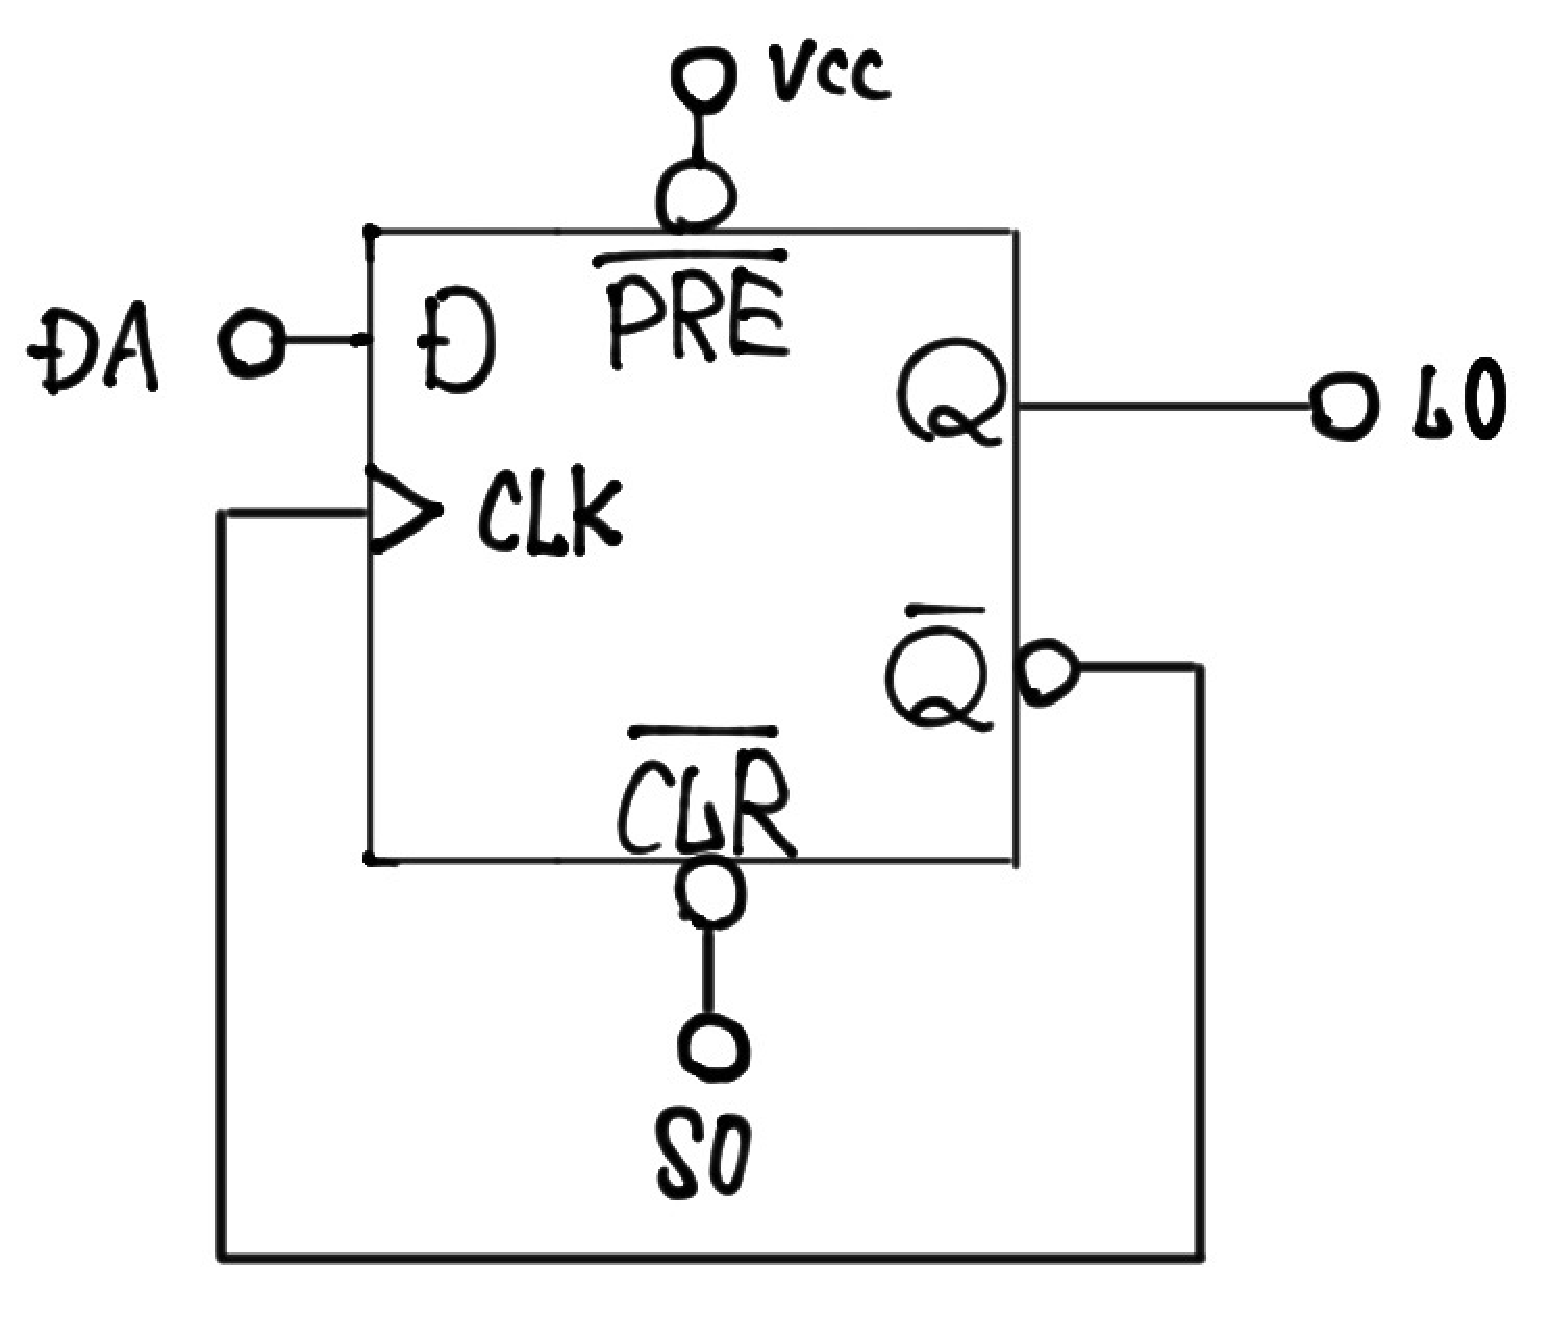
\includegraphics[width=8cm]{dffcirc2} \\%%% ファイル名
				\end {center}
			\end{minipage}
		\end{tabular}
		\caption{Dフリップフロップ回路の回路図}%%% 表題
		\label{fig:DFF}%%% ラベル
	\end{center}
\end{figure}
%
%
%
\begin{figure}[ht]
	\begin{center}
		\begin {tabular}{c}
			\begin{minipage}{8cm}
				\begin{center}
					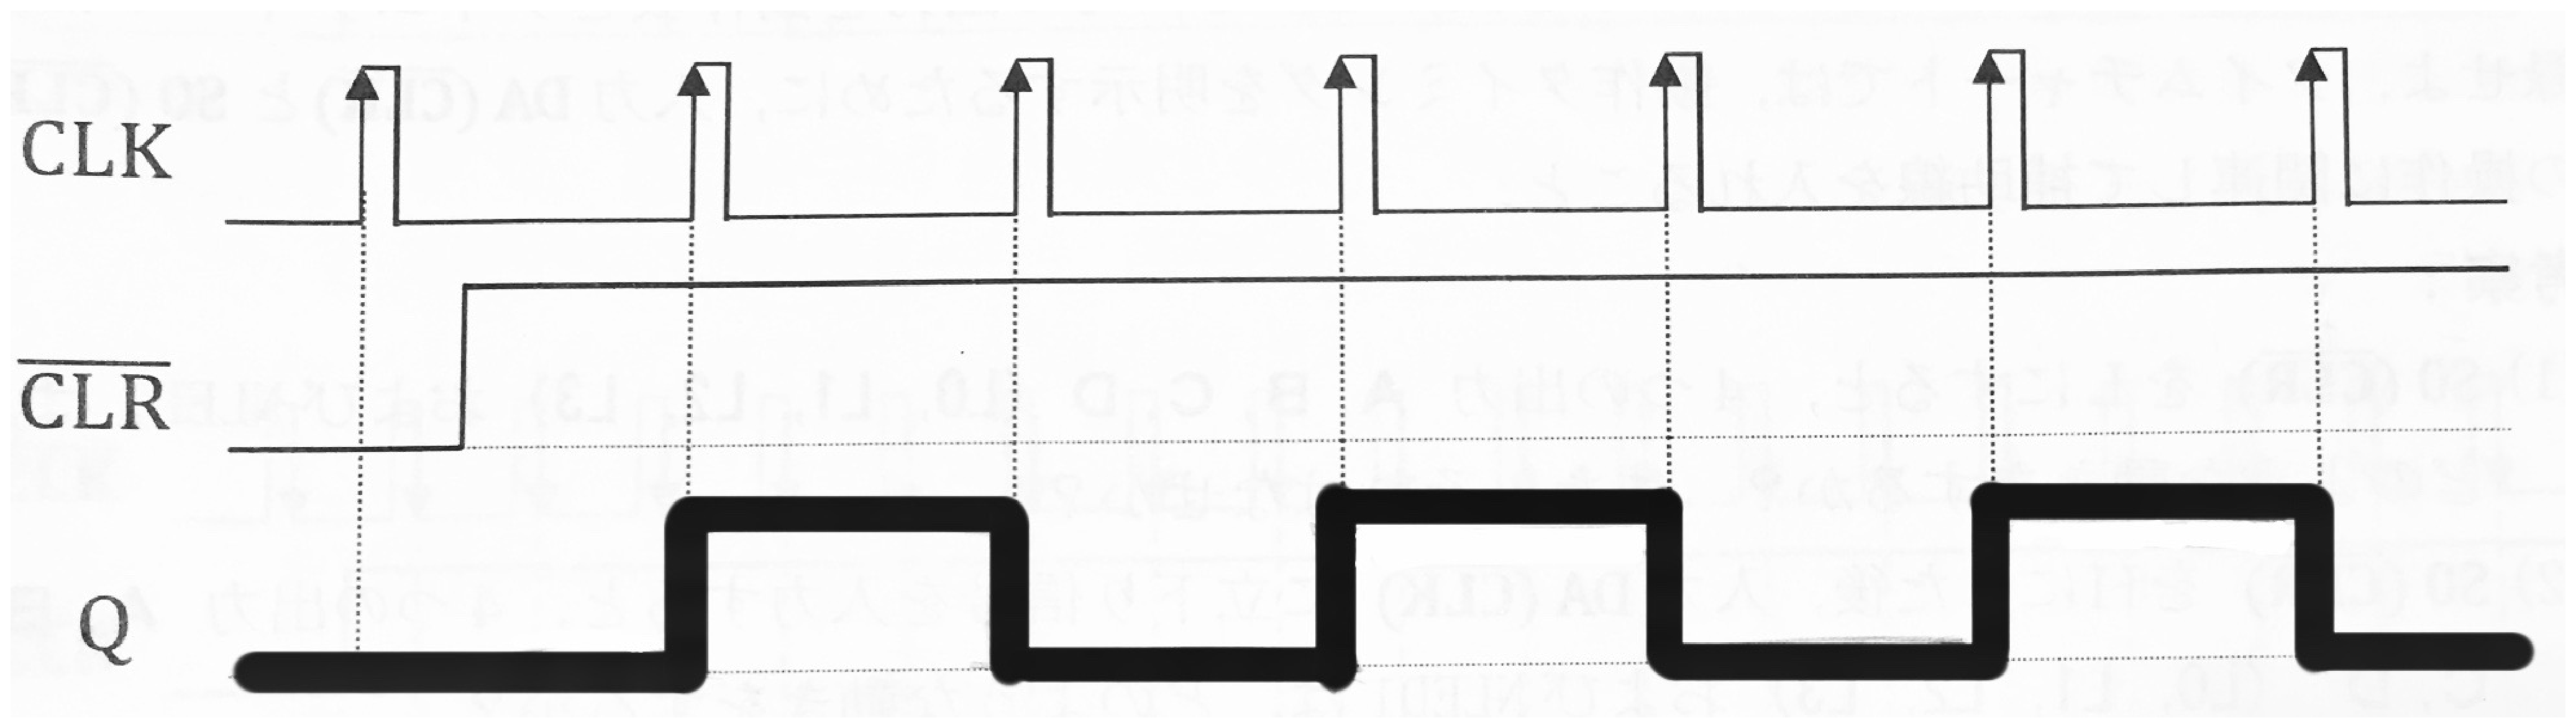
\includegraphics[width=8cm]{DFFTC} \\%%% ファイル名
				\end {center}
			\end{minipage}
		\end{tabular}
		\caption{Dフリップフロップ回路のタイムチャート}%%% 表題
		\label{fig:DFFTC}%%% ラベル
	\end{center}
\end{figure}
%
%
%
\begin{figure}[ht]
	\begin{center}
		\begin {tabular}{c}
			\begin{minipage}{12cm}
				\begin{center}
					\includegraphics[width=12cm]{16ctcir} \\%%% ファイル名
				\end {center}
			\end{minipage}
		\end{tabular}
		\caption{$16$進カウンタ回路の回路図}%%% 表題
		\label{fig:16Counter}%%% ラベル
	\end{center}
\end{figure}
%
%
%
\begin{figure}[ht]
	\begin{center}
		\begin {tabular}{c}
			\begin{minipage}{8cm}
				\begin{center}
					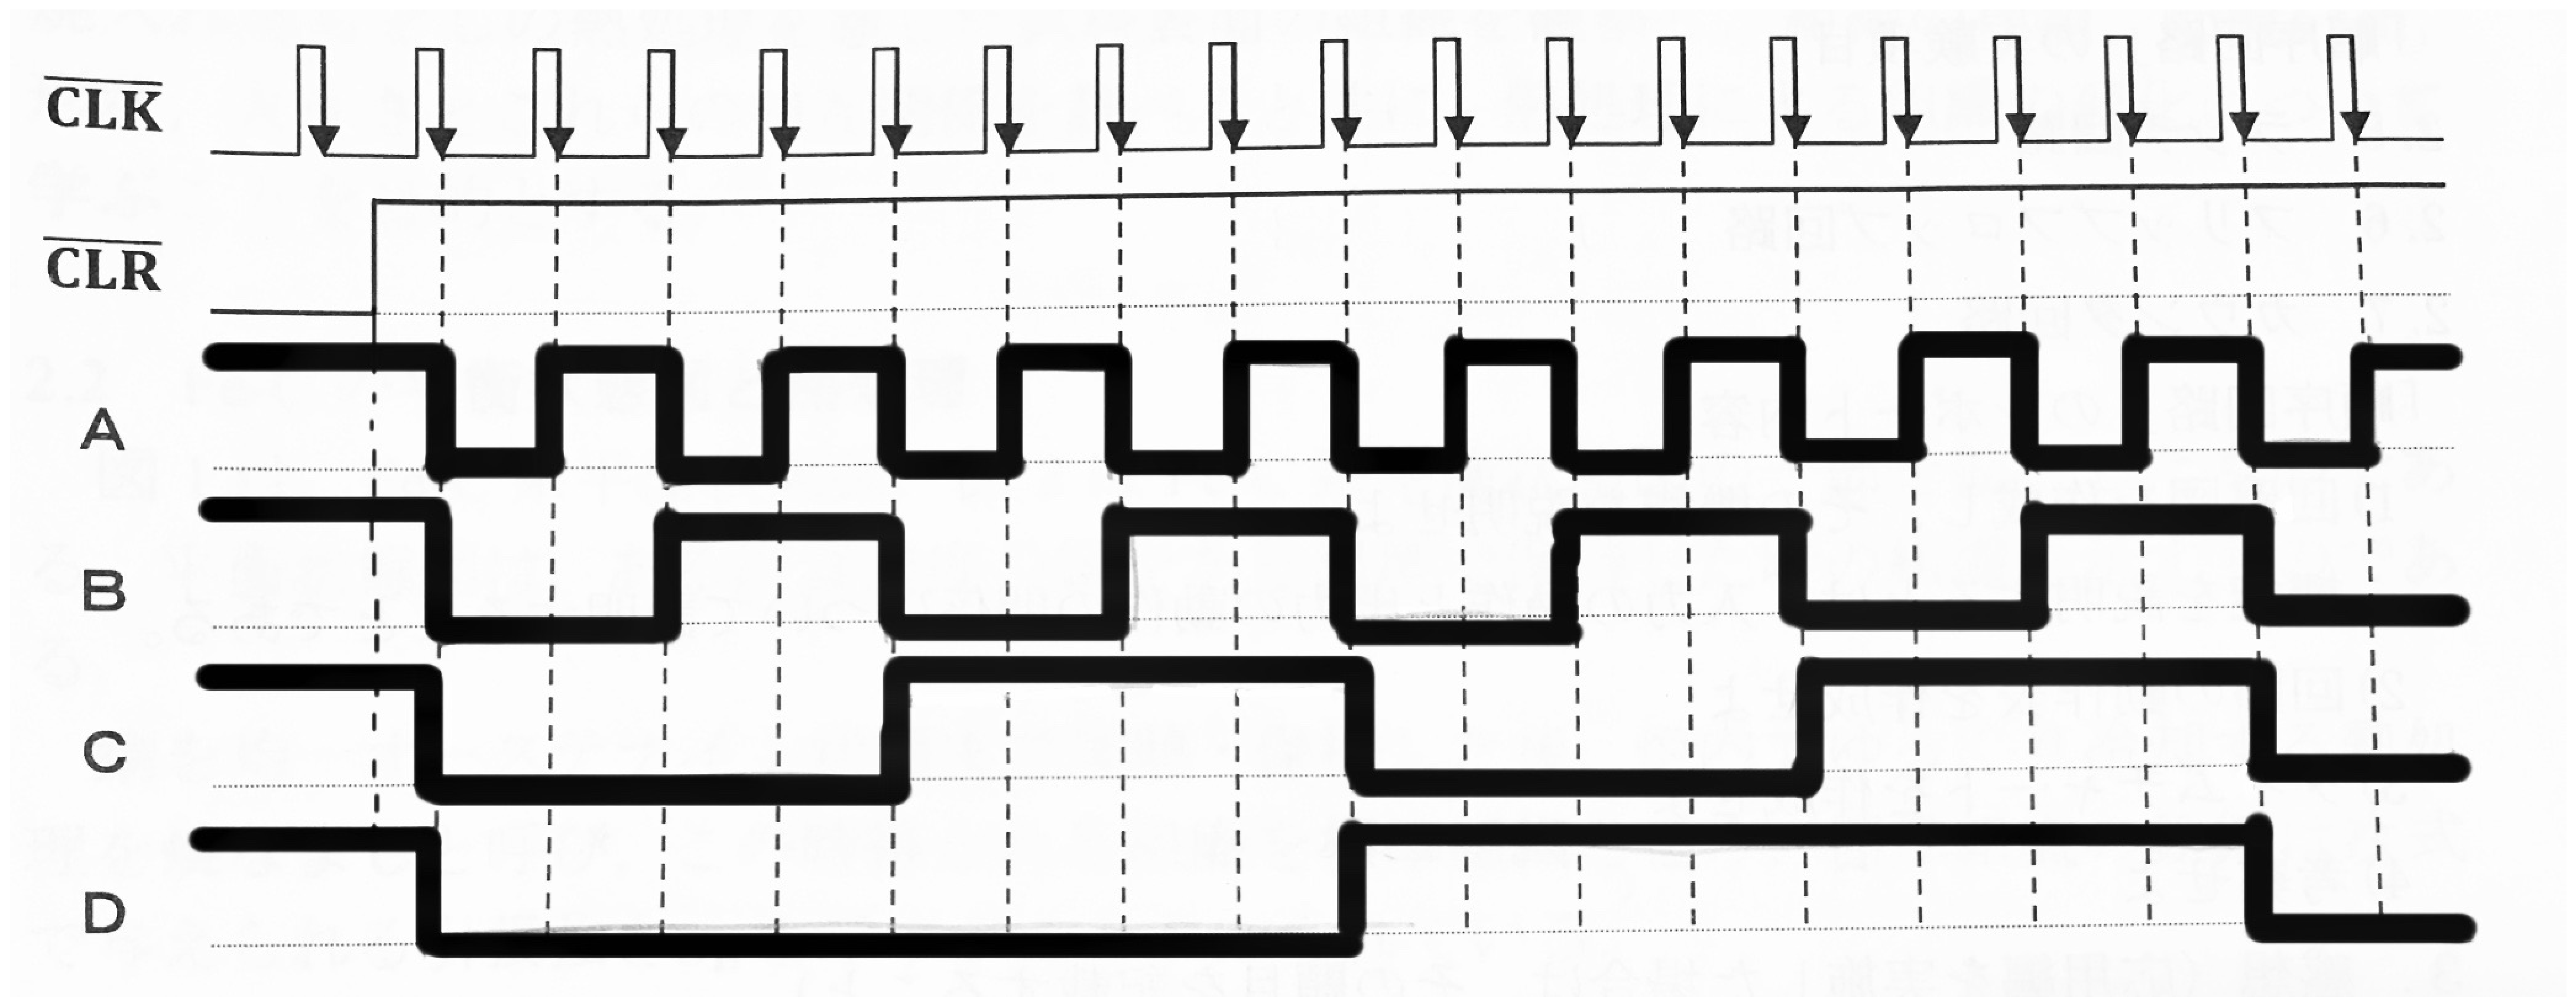
\includegraphics[width=8cm]{1111} \\%%% ファイル名
				\end {center}
			\end{minipage}
		\end{tabular}
		\caption{$16$進カウンタ回路のタイムチャート}%%% 表題
		\label{fig:16CounterTC}%%% ラベル
	\end{center}
\end{figure}

\end{document}
